\chapter{Results}
\label{chap:results}

Where appropriate the results of the \MFM and \SMVA are shown next to each other. As the \SMVA is a cross check to the background model and categorisation scheme, only results on exclusion power, observation significance and signal strength measurement are provided for the \SMVA. The results of couplings measurements and compatbility across channels and production mechanisms are shown only for the \MFM.

The results of the statistical hypothesis tests, which show an independent discovery of a Higgs like resonance near 125~\GeV, are shown first, after which measurements on the properties of the signal are discussed.

\section{Exclusion limits and $p$-value}

The exclusion limit for a \SM Higgs Boson is shown in Figure ~\ref{fig:res_exclusion} for the \MFM analysis (left) and the \SMVA analysis (right) for the combined 7 and 8~\TeV dataset. One can see that a \SM Higgs boson is largely disfavoured everywhere in the search range of $[110,150]$ apart from around 125~\GeV where a large excess is apparent. The $y$-axis is the amount of \SM signal excluded at 95\% confidence as a function of the hypothesised Higgs mass, \mH, on the $x$-axis. The black dashed line with the green and yellow bands respresents the expected exclusion, and the associated $\pm1\sigma$ and $\pm2\sigma$ error, if exactly the mean of the null hypothesis is observed. The solid black line represents the actual observation in data. It can be seen that the both the nominal \MFM analysis and the cross check \SMVA have similar exclusion power and the same observation.

\begin{figure}
  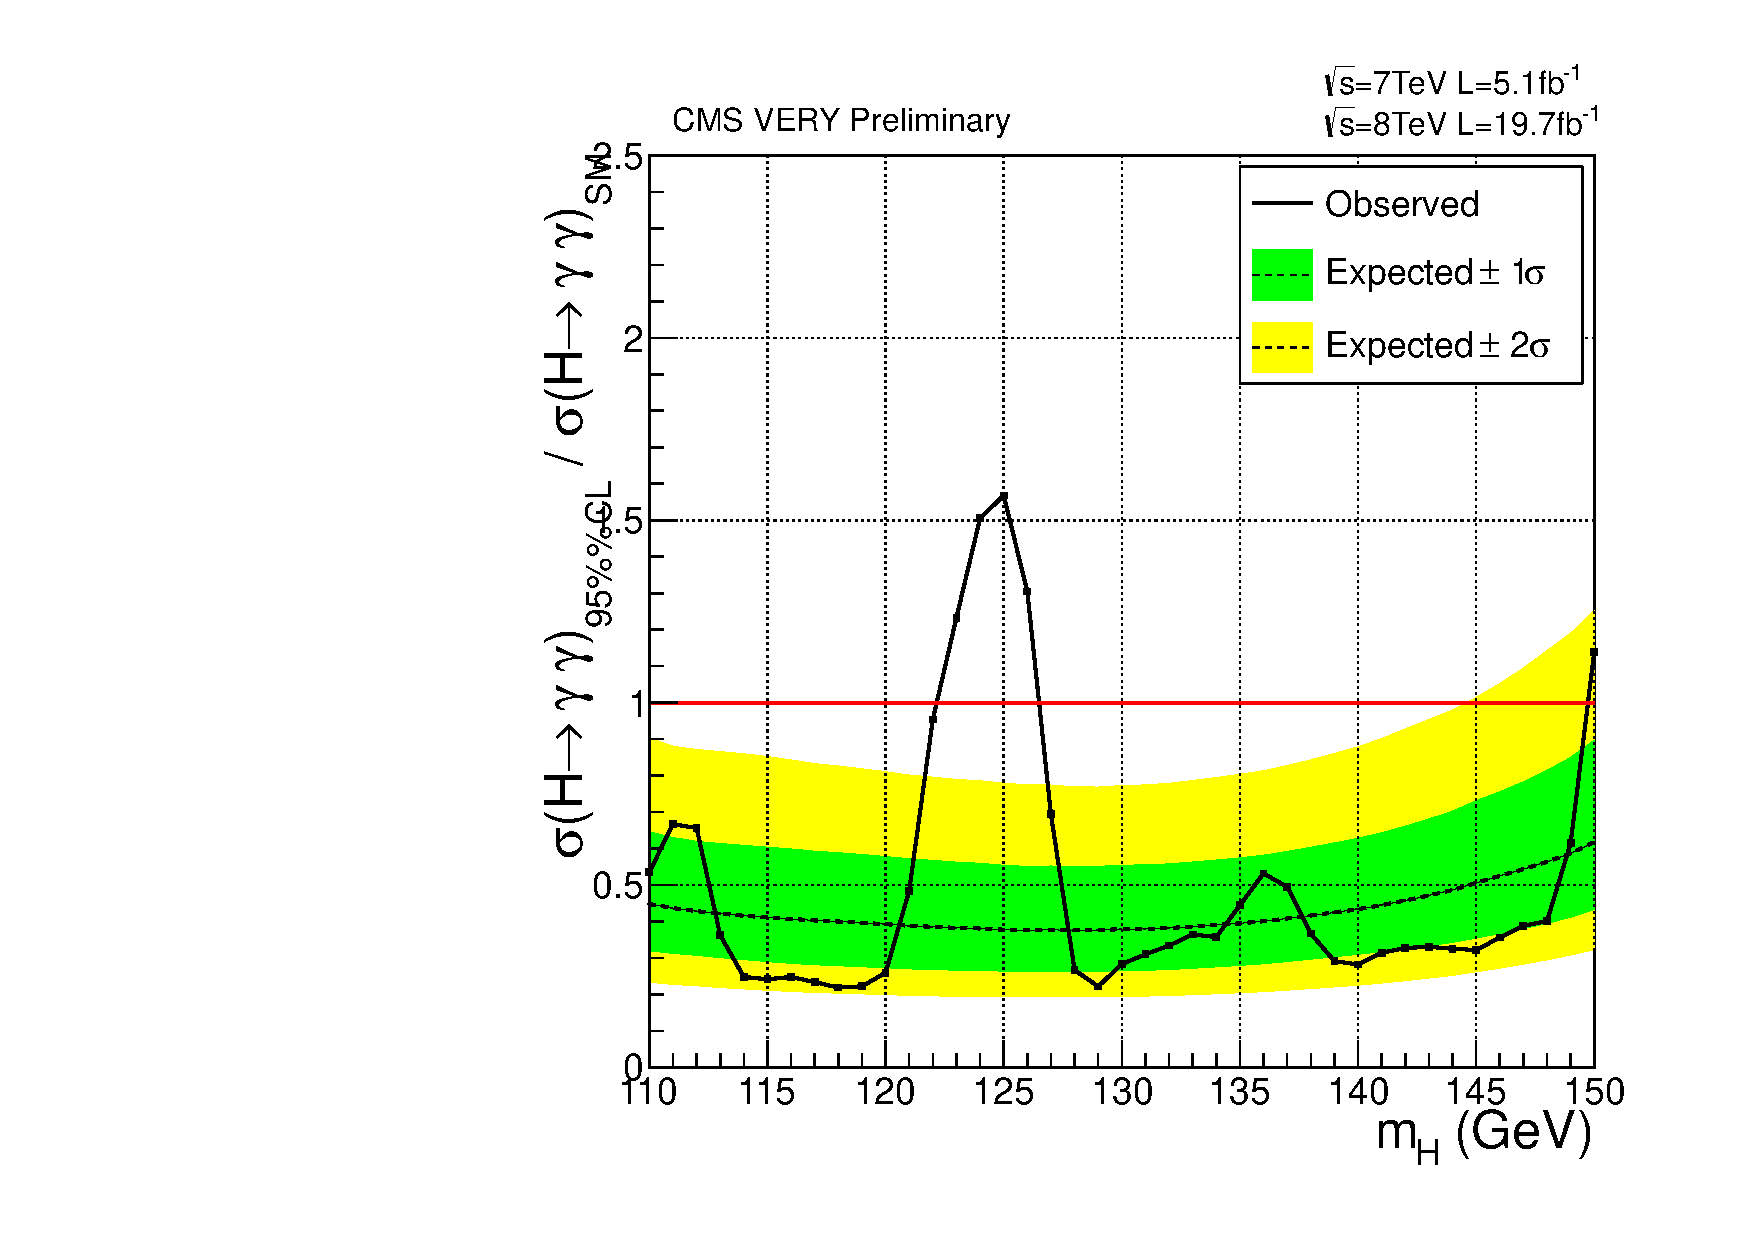
\includegraphics[width=0.49\textwidth]{analysis/plots/results/obslimit.pdf}
  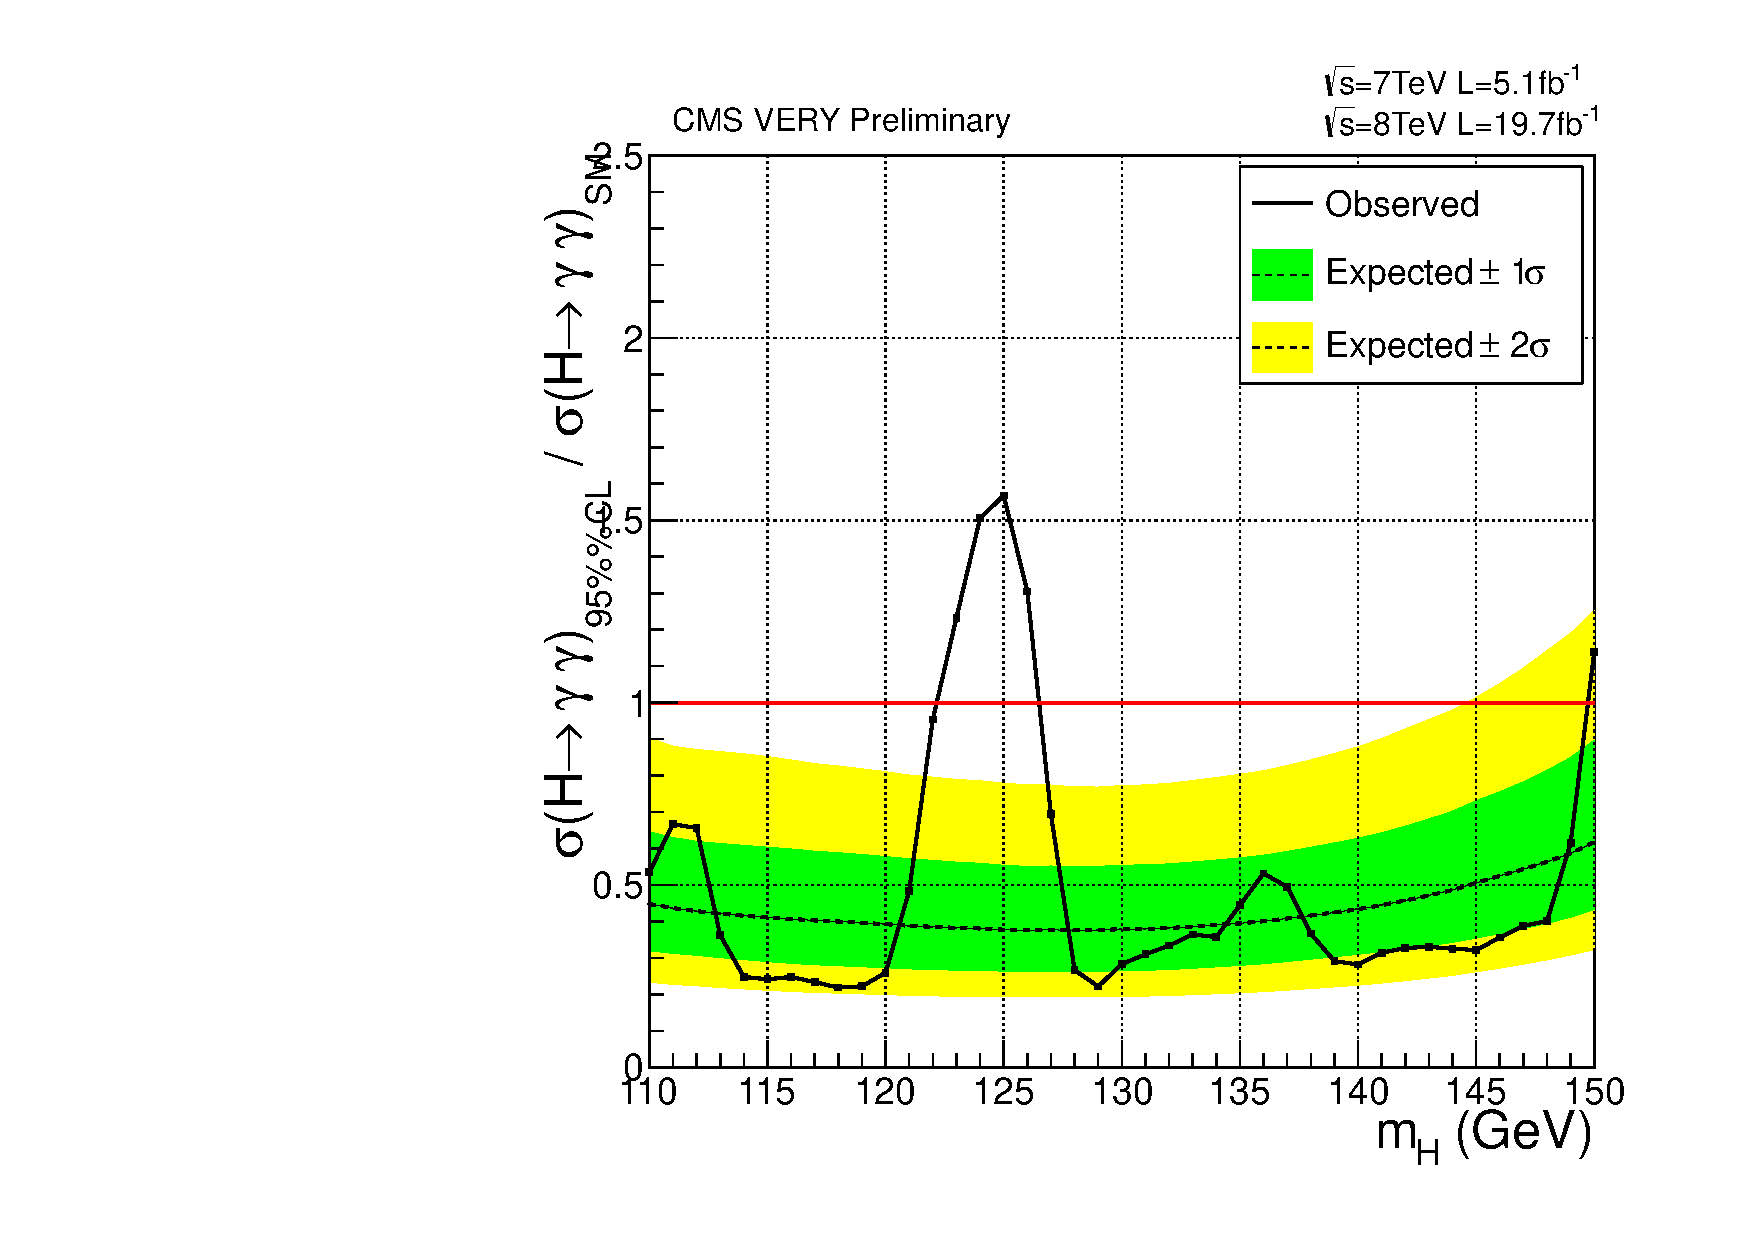
\includegraphics[width=0.49\textwidth]{analysis/plots/results/obslimit_sideband.pdf}
  \caption[The expected and observed exclusion limits for a \SM Higgs boson at 95\& confidence level]{The expected and observed exclusion limits for a \SM Higgs boson at 95\% confidence level. The dashed line shows the expectated exclusion if exactly the mean of the null hypothesis is observed with its error at $1\sigma$ (green) and $2\sigma$ (yellow). The solid black line shows the observed exclusion. The results are shown for the nominal \MFM analysis (left) and the cross check \SMVA (right) when combining both the 7 and 8~\TeV datasets. A \SM Higgs boson is disfavoured at 95\% everywhere apart from where there is a large excess around 125~\GeV. \plotupdate}
  \label{fig:res_exclusion}
\end{figure}

In order to quantify the significance of this excess the observed local $p$-value is shown as a function of the hypothesised Higgs mass, \mH, in Fig.~\ref{fig:res_pvalue} for both the 7~\TeV (blue line) and 8~\TeV (red line) datasets seperately and the combination (black line). It is clear there is a significant excess in both subsets of data at approximately the same mass and the quantity of the excess is apparent in both the \MFM and \SMVA analyses. The local $p$-value for the \MFM using the combined 7 and 8~\TeV datasets at \mH=124.7~\GeV (the mass with the most significant excess) is 5.7$\sigma$ where 5.2$\sigma$ is the expectation for a \SM Higgs boson. This constitutes a standalone discovery of a Higgs like resonance around 125~\GeV.

\begin{figure}
  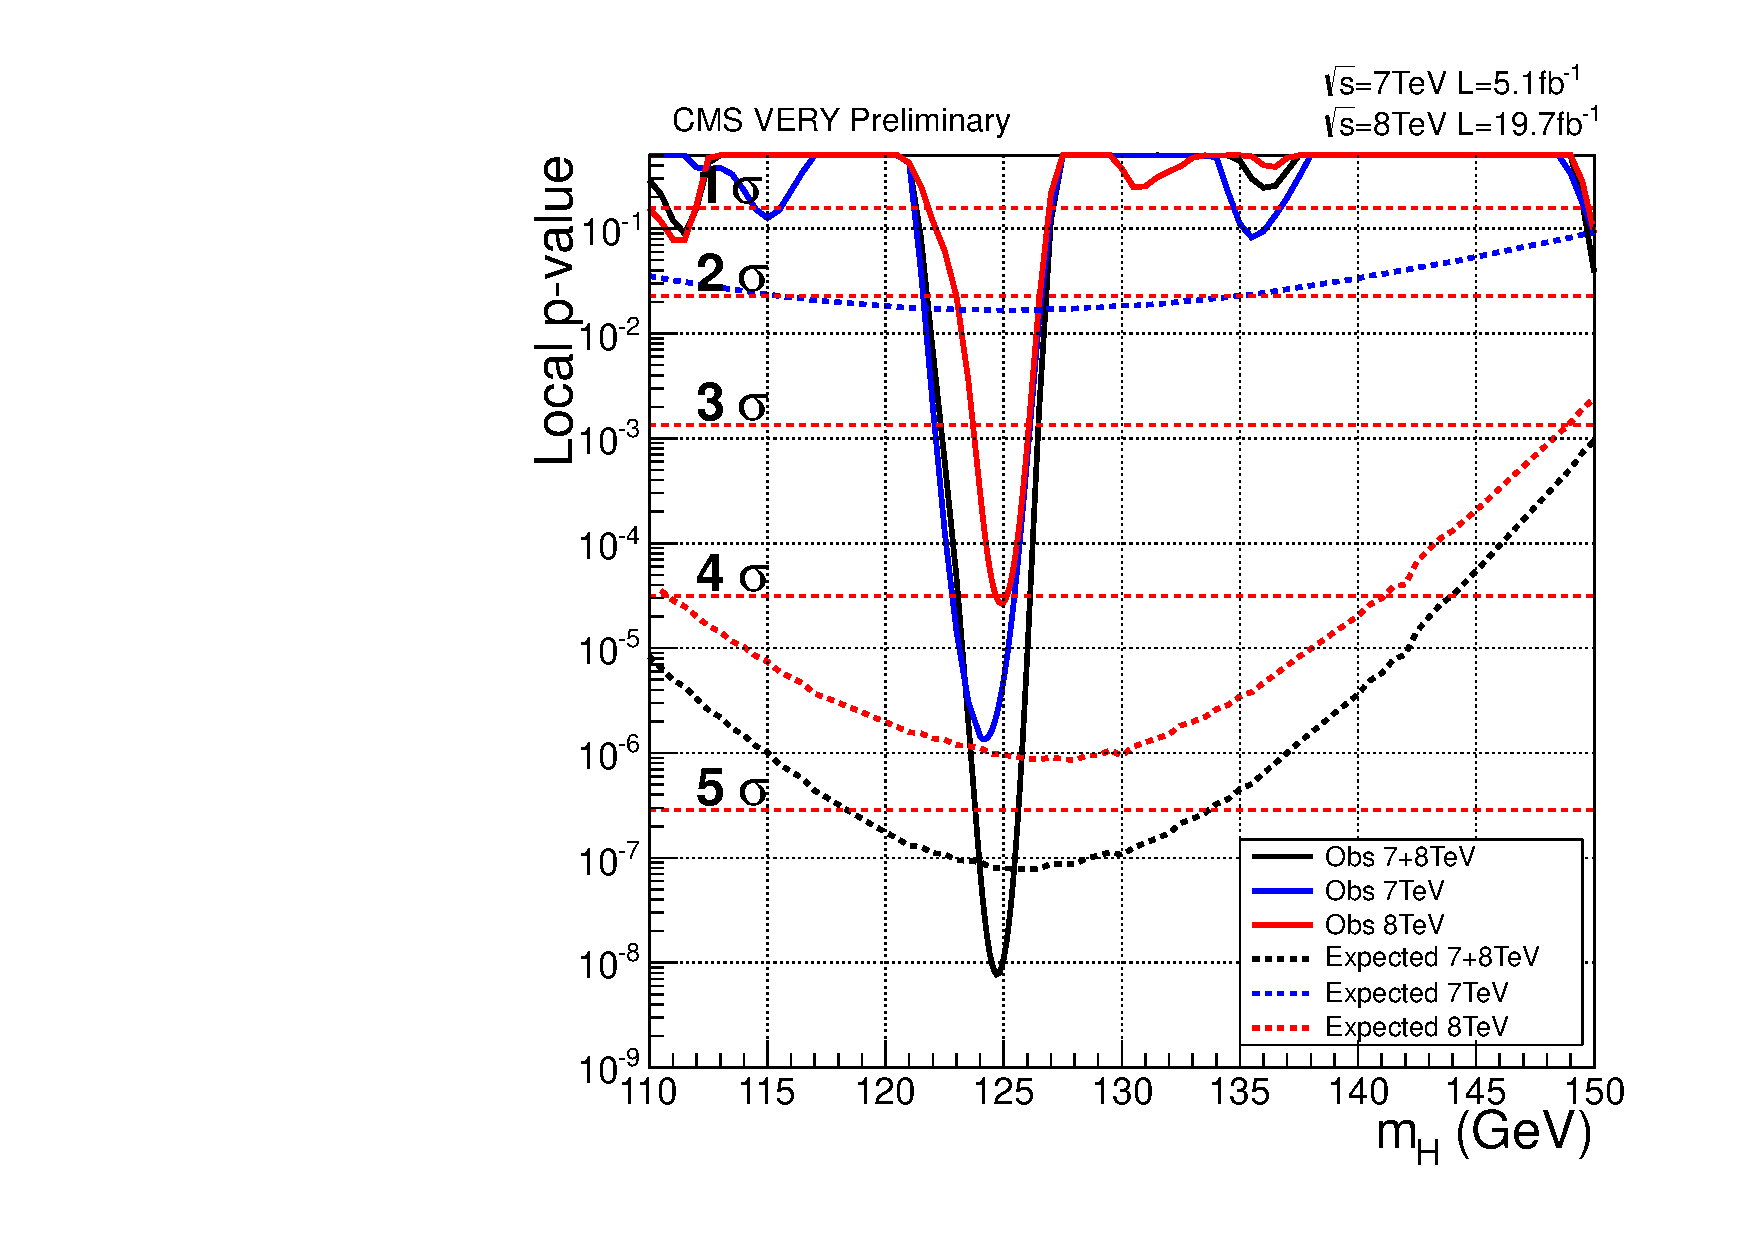
\includegraphics[width=0.49\textwidth]{analysis/plots/results/obspvalue.pdf}
  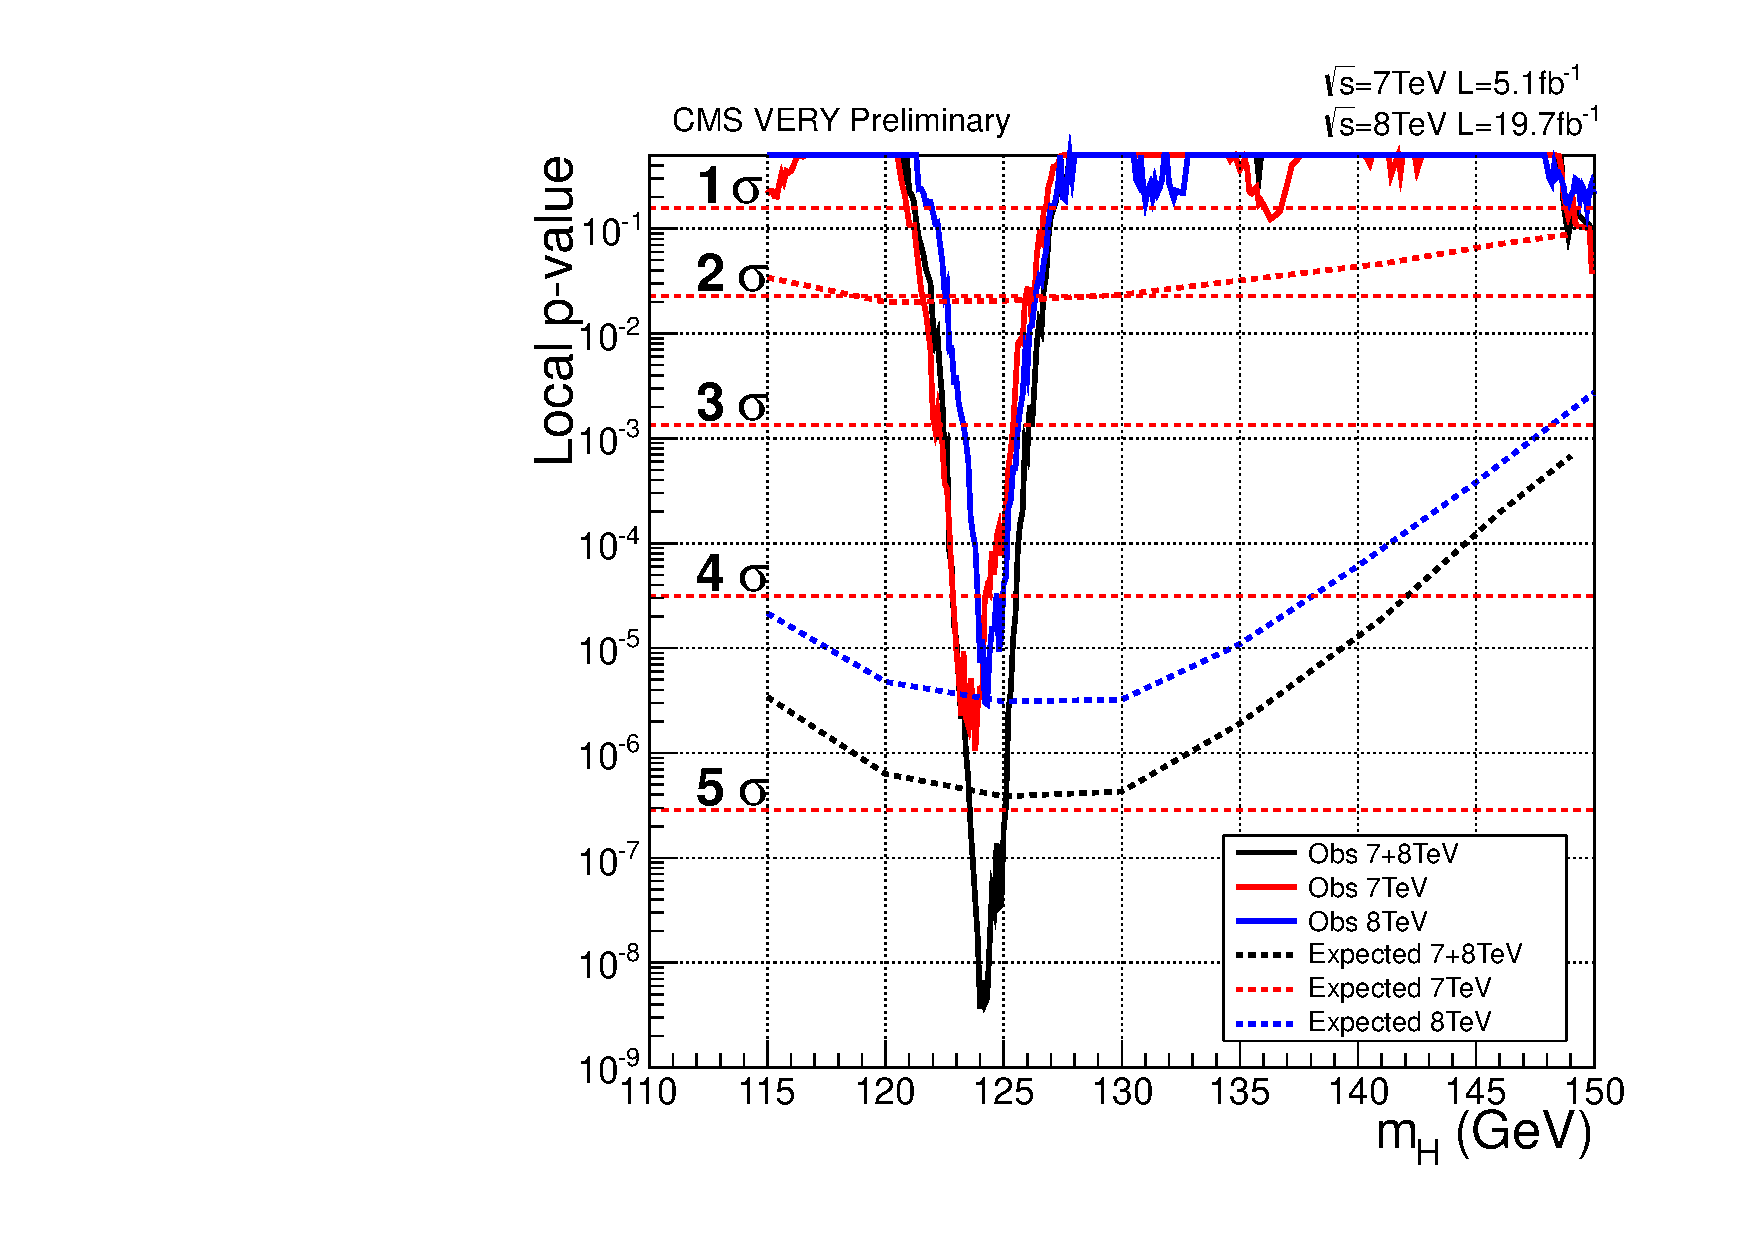
\includegraphics[width=0.49\textwidth]{analysis/plots/results/obspvalue_sideband.pdf}
  \caption[The expected and observed local $p$-value to reject the background hypothesis]{The expected (dashed lines) and observed (solid lines) local $p$-value to reject the background only hypothesis as a function of the hypothesised Higgs mass, \mH. The 7~\TeV (blue lines) and 8~\TeV (red lines) results are show separately along with the combination (black lines). The results are shown for the nominal \MFM analysis (left) and the cross check \SMVA (right). The observed $p$-value in the \MFM at the most significant point is 5.7$\sigma$ (\mH=124.7~\GeV) given a \SM expectation of $5.2\sigma$. \plotupdate}
  \label{fig:res_pvalue}
\end{figure}

\section{Measurement of physicsal parameters}

The best fit value of the signal strength modifier, $\mu=\musm$, is shown as a function of the hypothesis Higgs mass, \mH, in Fig.~\ref{fig:res_mumh} for the combined 7 and 8~\TeV dataset. As expected this follows very similarly the shape of the observed exclusion in Fig.~\ref{fig:res_exclusion} and shows that the observed boson is very compatible with a \SM Higgs, i.e.~the observed value of $\mu$ is within $1\sigma$ of the \SM expectation, $\mu=1$. 

\begin{figure}
  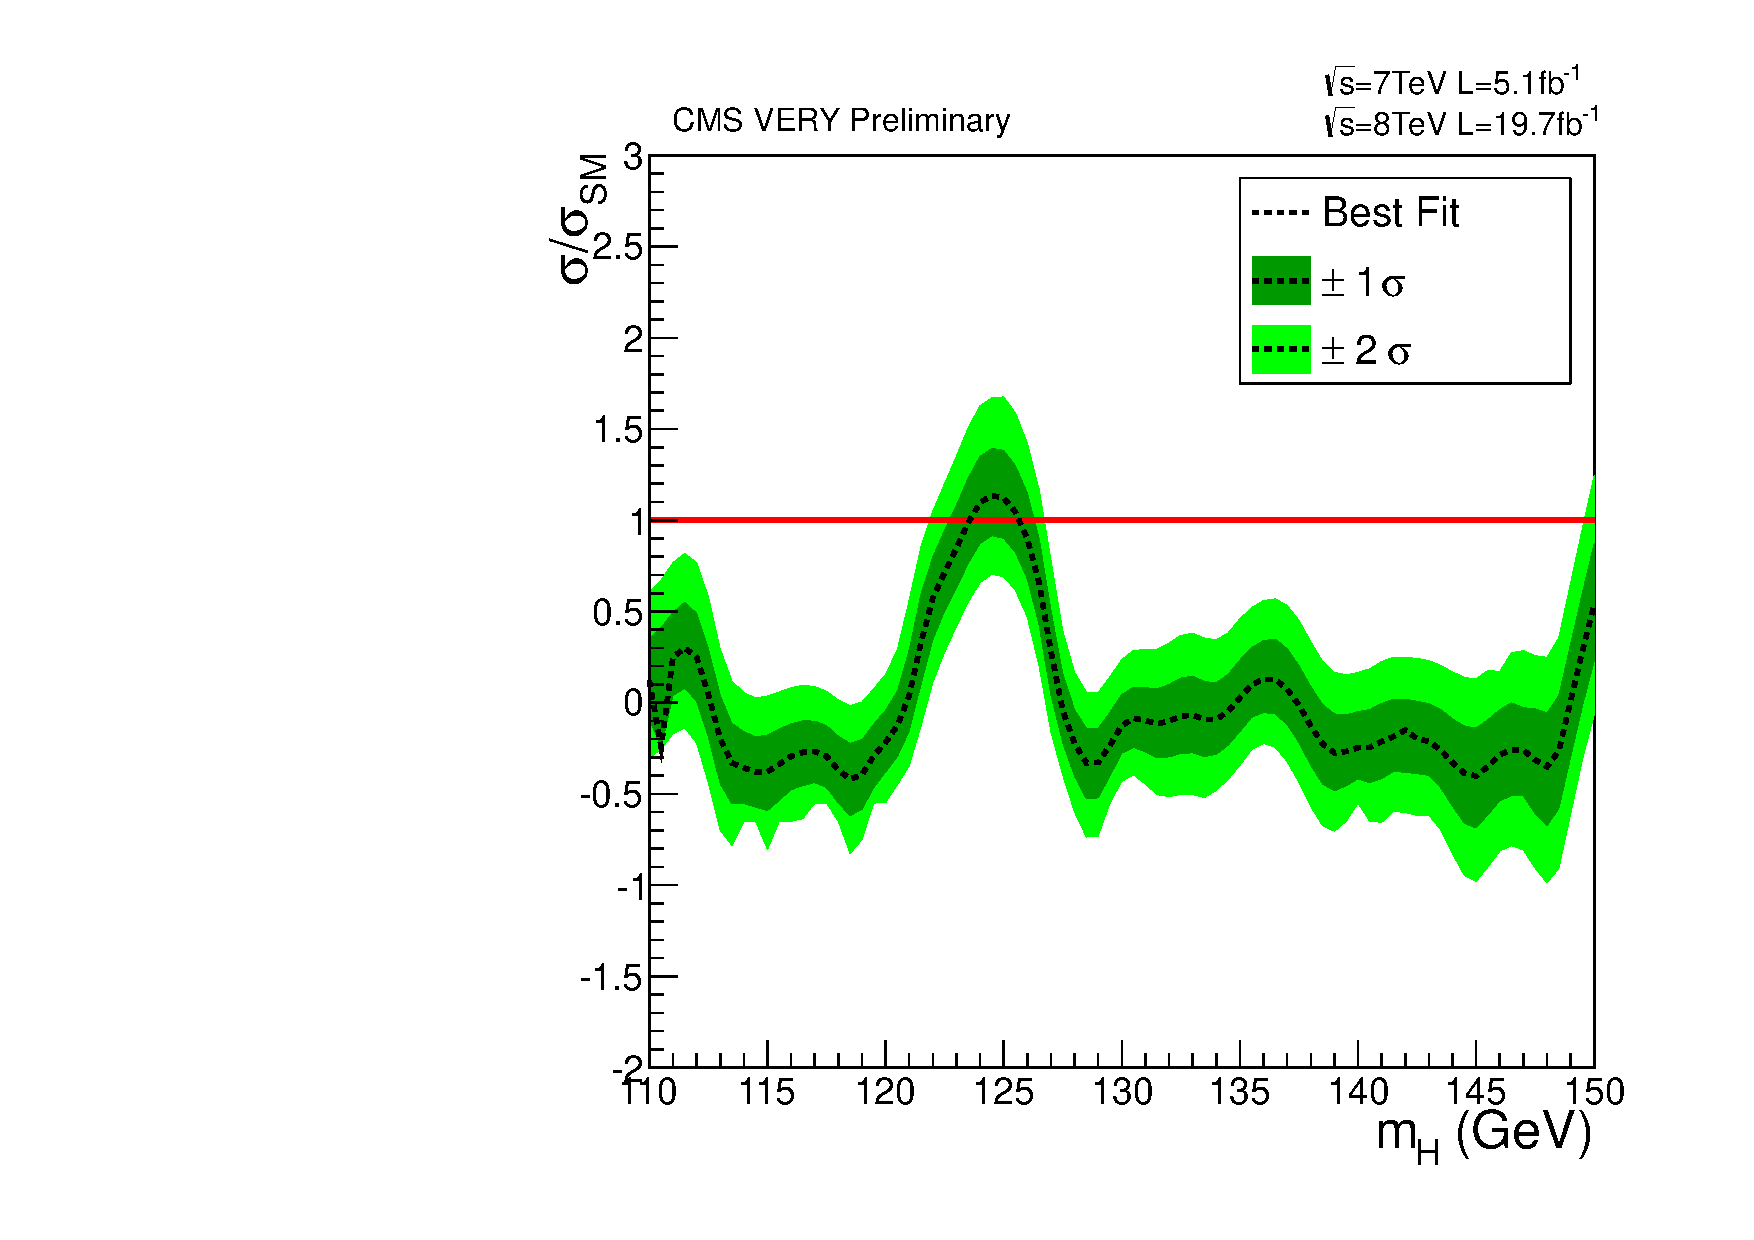
\includegraphics[width=0.49\textwidth]{analysis/plots/results/obsmumh.pdf}
  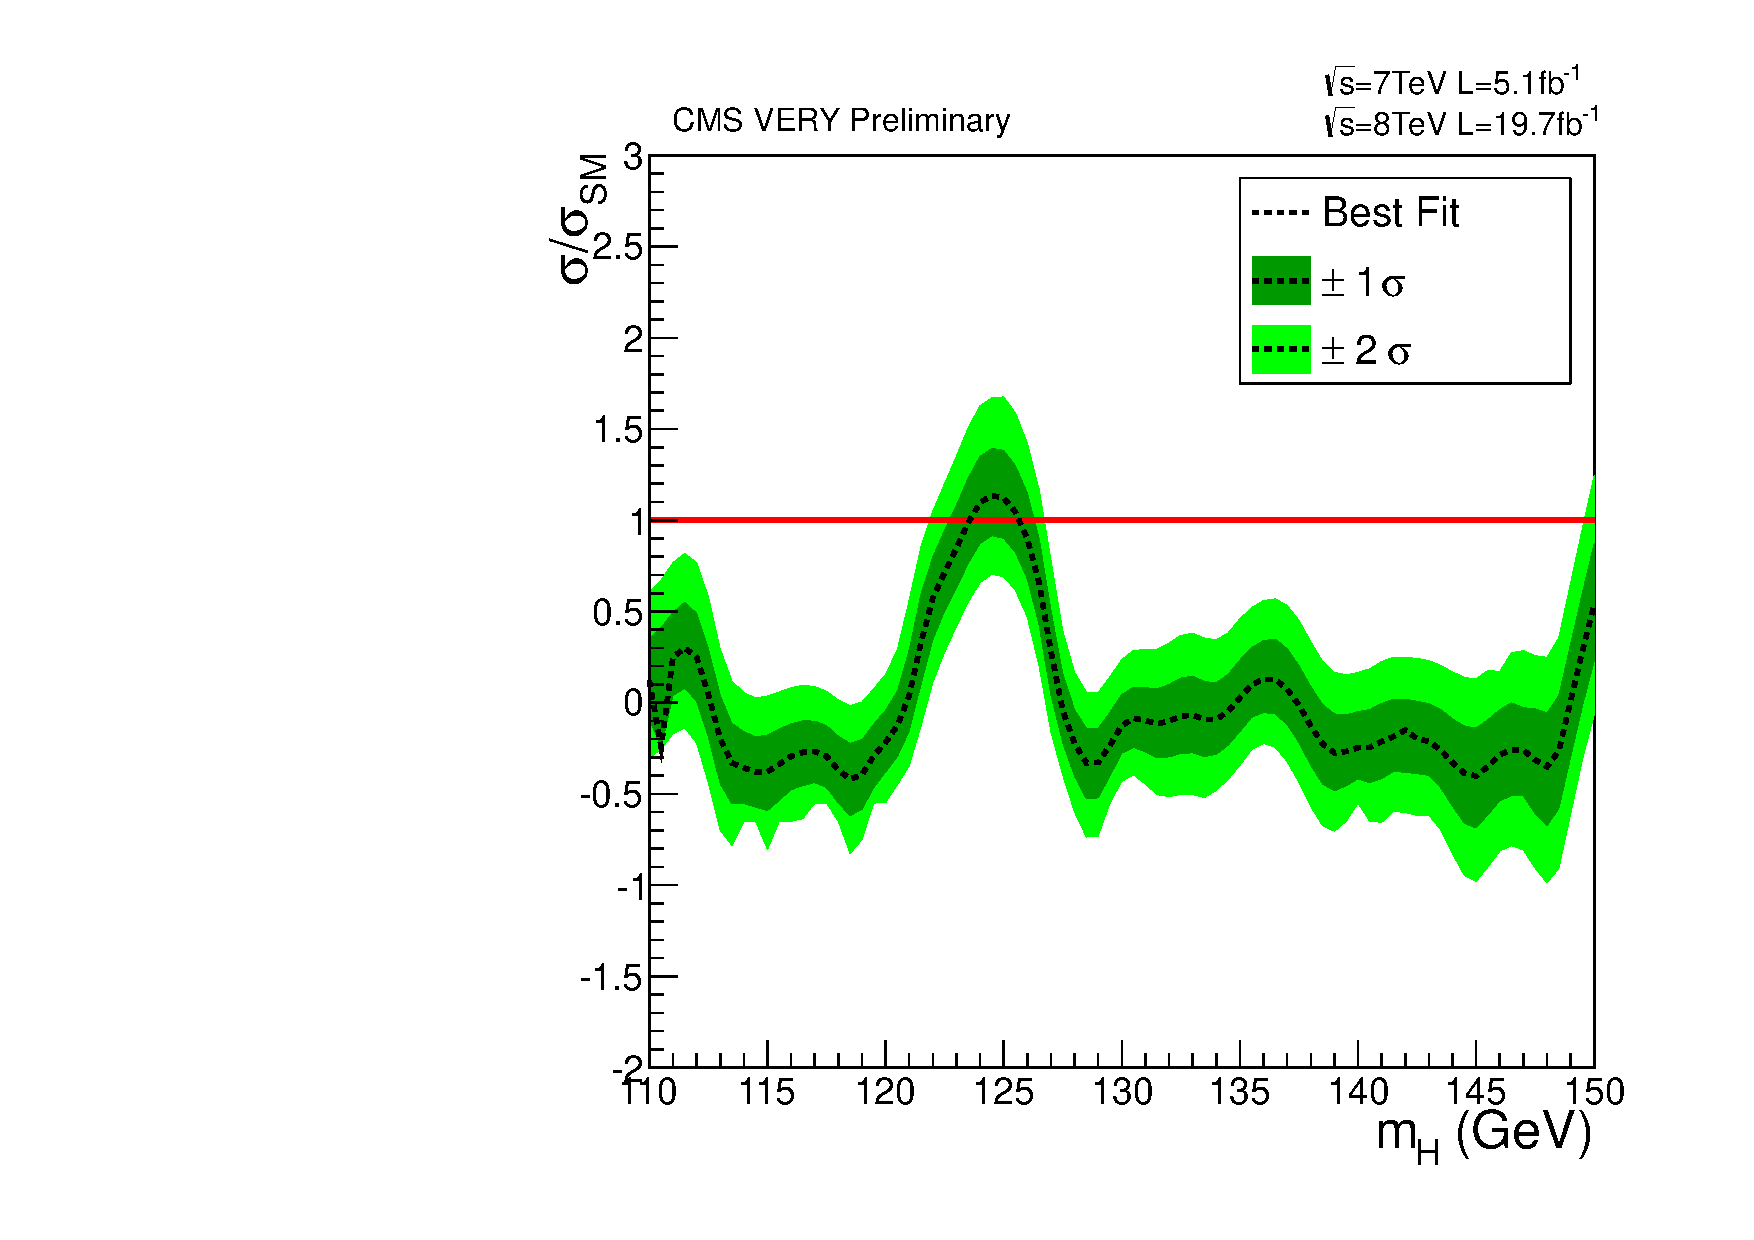
\includegraphics[width=0.49\textwidth]{analysis/plots/results/obsmumh_sideband.pdf}
  \caption[The observed best fit value of the signal strength modifier $\mu$]{The observed best fit value of the signal strength modifier, $\mu=\musm$, as a function of the hypothesised Higgs mass \mH when using the combined 7 and 8~\TeV datasets. The $\pm1\sigma$ and $\pm2\sigma$ error bands are shown as the dark and light green bands respectively. Results are shown for the nominal \MFM analysis (left) and the cross check \SMVA analysis (right). \plotupdate.}
  \label{fig:res_mumh}
\end{figure}

Figure~\ref{fig:res_muscan} shows the one dimensional \NLL scan of $\mu$ when the Higgs mass \mH is profiled. The hypothesis mass, \mH, is left floating in the fit as there is no \textit{a priori} knowledge of its value. The likelihood curves are shown for the 7 and 8~\TeV datasets separately, blue and red lines respectively, as well as for the combination, black line. The \SM expectation is shown as the dashed lines. One can see that the results are very consistent between the \MFM (left) and the \SMVA (right). There is some distance between the measurement made using the 7~\TeV dataset (blue line) and the 8~\TeV dataset (red line) but they are consistent at $<2\sigma$ level and it is quite reasonbale to imagine an upward fluctutation in the data at 7~\TeV and a downward fluctutaion at 8~\TeV. When combining the two datasets the best fit value comes out very close to the \SM expectation of $\mu=1$ so certainly an interesting area for future measurements with more data in the \Hgg channel is where this value goes. The best fit values of $\musm$ with their errors (and the mass at which the best fit is found) are summarised for each of the datasets using the \MFM analysis in Table~\ref{tab:res_mu}.

\begin{figure}
  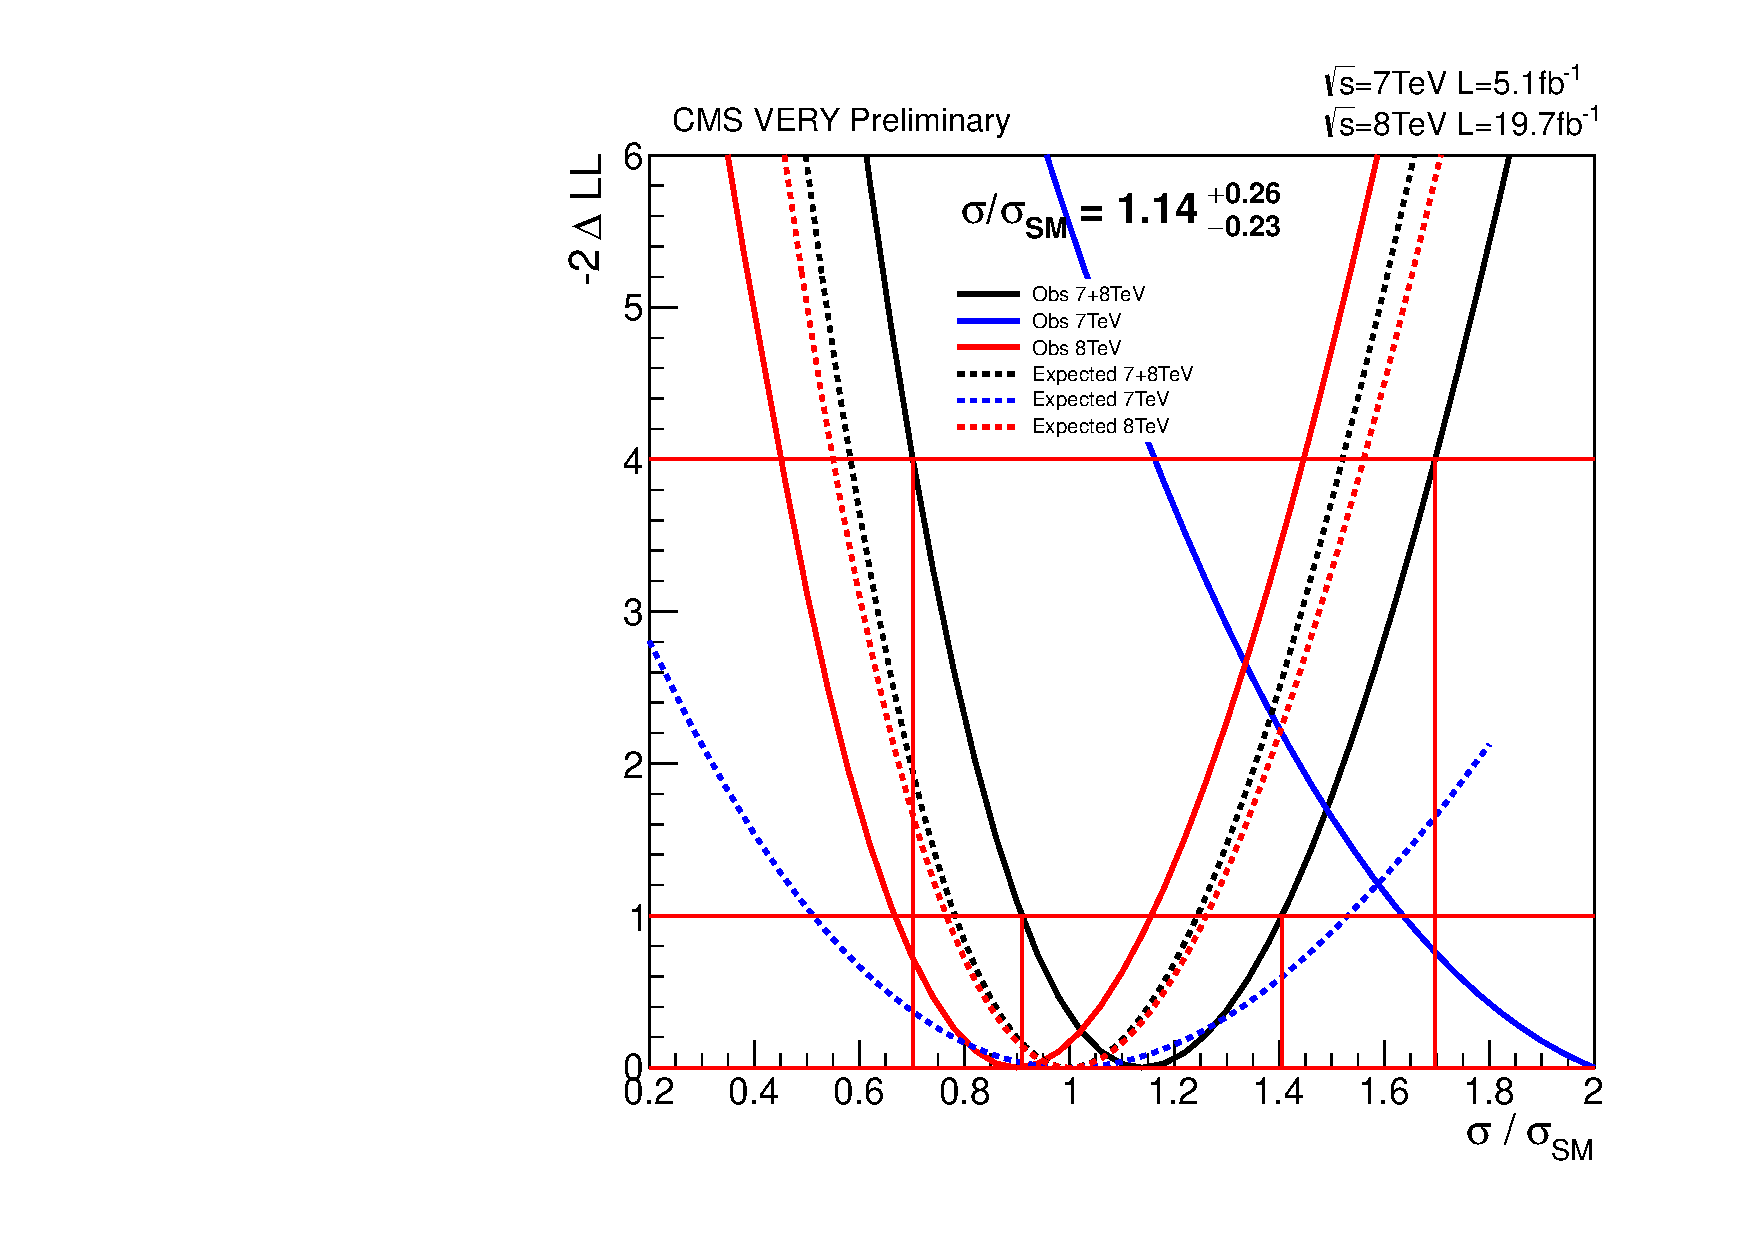
\includegraphics[width=0.49\textwidth]{analysis/plots/results/obsmu.pdf}
  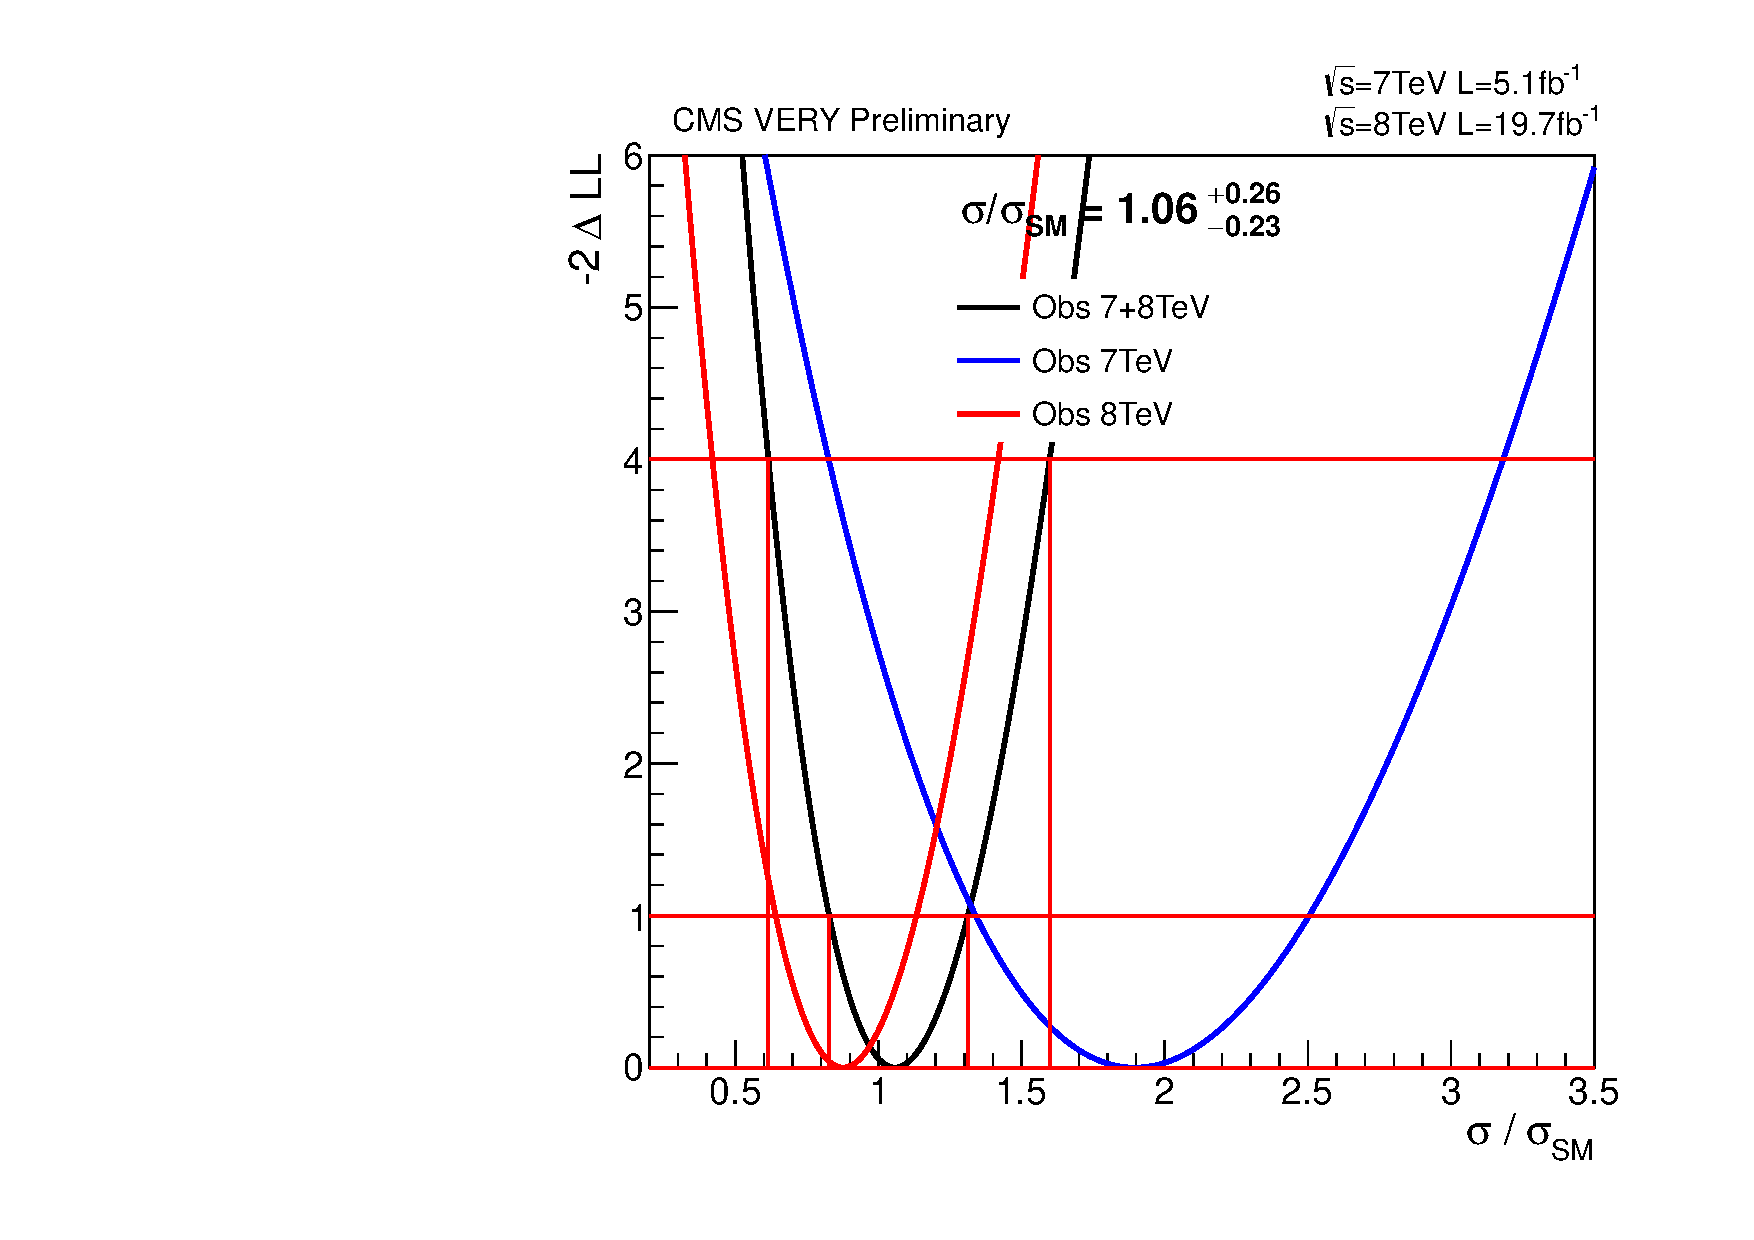
\includegraphics[width=0.49\textwidth]{analysis/plots/results/obsmu_sideband.pdf}\\
  \caption[The 1D \NLL scan of the signal strenght modifier $\mu$]{The one dimensional \NLL scan of the signal strength modifier, $\mu=\musm$, when the hypothesis Higgs mass, \mH, is profiled in the fit. The \SM expectation and the observation in data are shown as the dashed and solid lines respectively. The results are shown for the 7~\TeV (blue), the 8~\TeV (red) and combined (black) datasets using the \MFM analysis (left) and the \SMVA analysis (right). The observed best fit value for the nominal \MFM analysis is $\musm=1.14^{+0.26}_{-0.23}$.}
  \label{fig:res_muscan}
\end{figure}

\begin{table}
    \caption{\label{tab:res_mu} The values of the best fit signal
      strength, $\musm$, when \mH is profiled, for the 7\TeV, 8\TeV, and combined datasets. 
      The value of \mH\ at which the best fit occurs is also given.
      }
  \begin{center}
    \begin{tabular}{l|c|c}
      & $\musm$  & $\mH$ (GeV)       \\  \hline
      7 TeV  & $2.22^{+0.62}_{-0.55}$ & 124.2  \\ 
      8 TeV  & $0.91^{+0.26}_{-0.23}$ & 124.9  \\ \hline
      7 + 8 TeV & $1.14^{+0.27}_{-0.23}$ & 124.7  \\ 
    \end{tabular}
    \end{center}
\end{table}

The following measurements focus on the properties of the observed signal and are consequently only shown for the \MFM analysis. The two most important physical parameters to measure in the signal are the overall rate, $\mu$, and the mass, \mH. We have seen the 1D \NLL scan of the signal strength, $\mu$, when \mH is profiled. The result of doing a two dimensional \NLL scan in both the parameters simultaneously is shown on the left hand side of Fig.~\ref{fig:res_mumh2} for the combined 7+8~\TeV dataset. The overall best fit (see Table~\ref{tab:res_mu}) is represented by the black cross where the solid and dashed lines correspond to the $1\sigma$ and $2\sigma$ error contours. For a standalone measurement of the mass of the observed particle it is undesirable to constrain the signal resonance to have exactly \SM like couplings and production rates. Consequently, when measuring the mass, the overall signal rate is allowed to scale in terms of the production from fermion couplings, \RF, and from boson couplings, \RV (see Eq.~\ref{eq:rvrf}). The one dimensional \NLL scan of the observed mass is shown on the right hand side of Fig.~\ref{fig:res_mumh2} for the combined 7+8~\TeV dataset when profiling the \RV and \RF signal strengths. This is shown when including all uncertainties (black) and when considering just the statistical uncertainties in the data (blue). It should be noted that in principal the best fit mass when scanning the two dimensions of $\mu$ and \mH (Fig.~\ref{fig:res_mumh2} left) does not necessarily have to be the same as the mass when scanning one dimension \mH but floating two other parameters, \RV and \RF (Fig.~\ref{fig:res_mumh2} right). However, in practise they come out almost identical because, as is shown below, the coupling strength parameters \RV and \RF come out very close to the \SM expectation. The observed best fit mass of the boson is found to be $\mH=124.73\pm0.34$(stat)$\pm0.15$(syst)~\GeV. 

\begin{figure}
  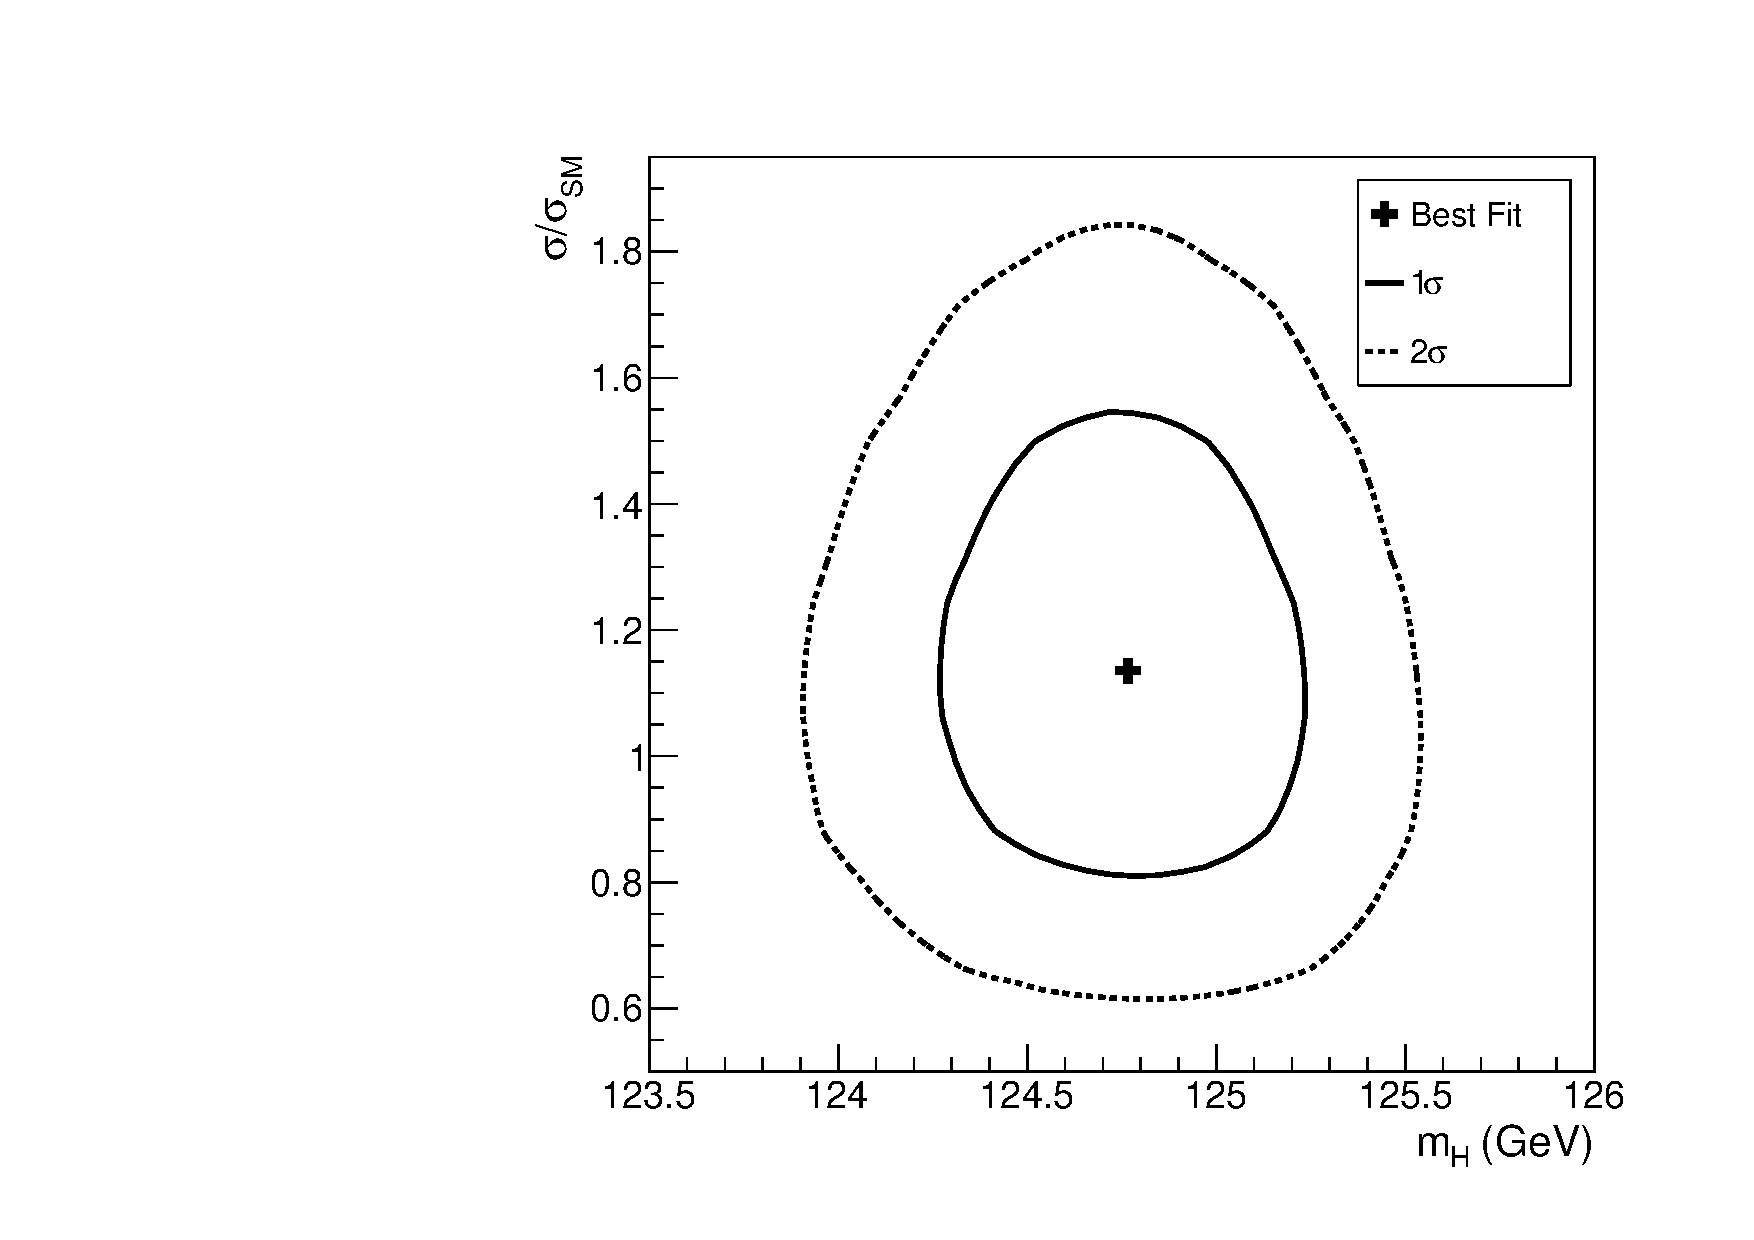
\includegraphics[width=0.49\textwidth]{analysis/plots/results/obsmumh2D.pdf}
  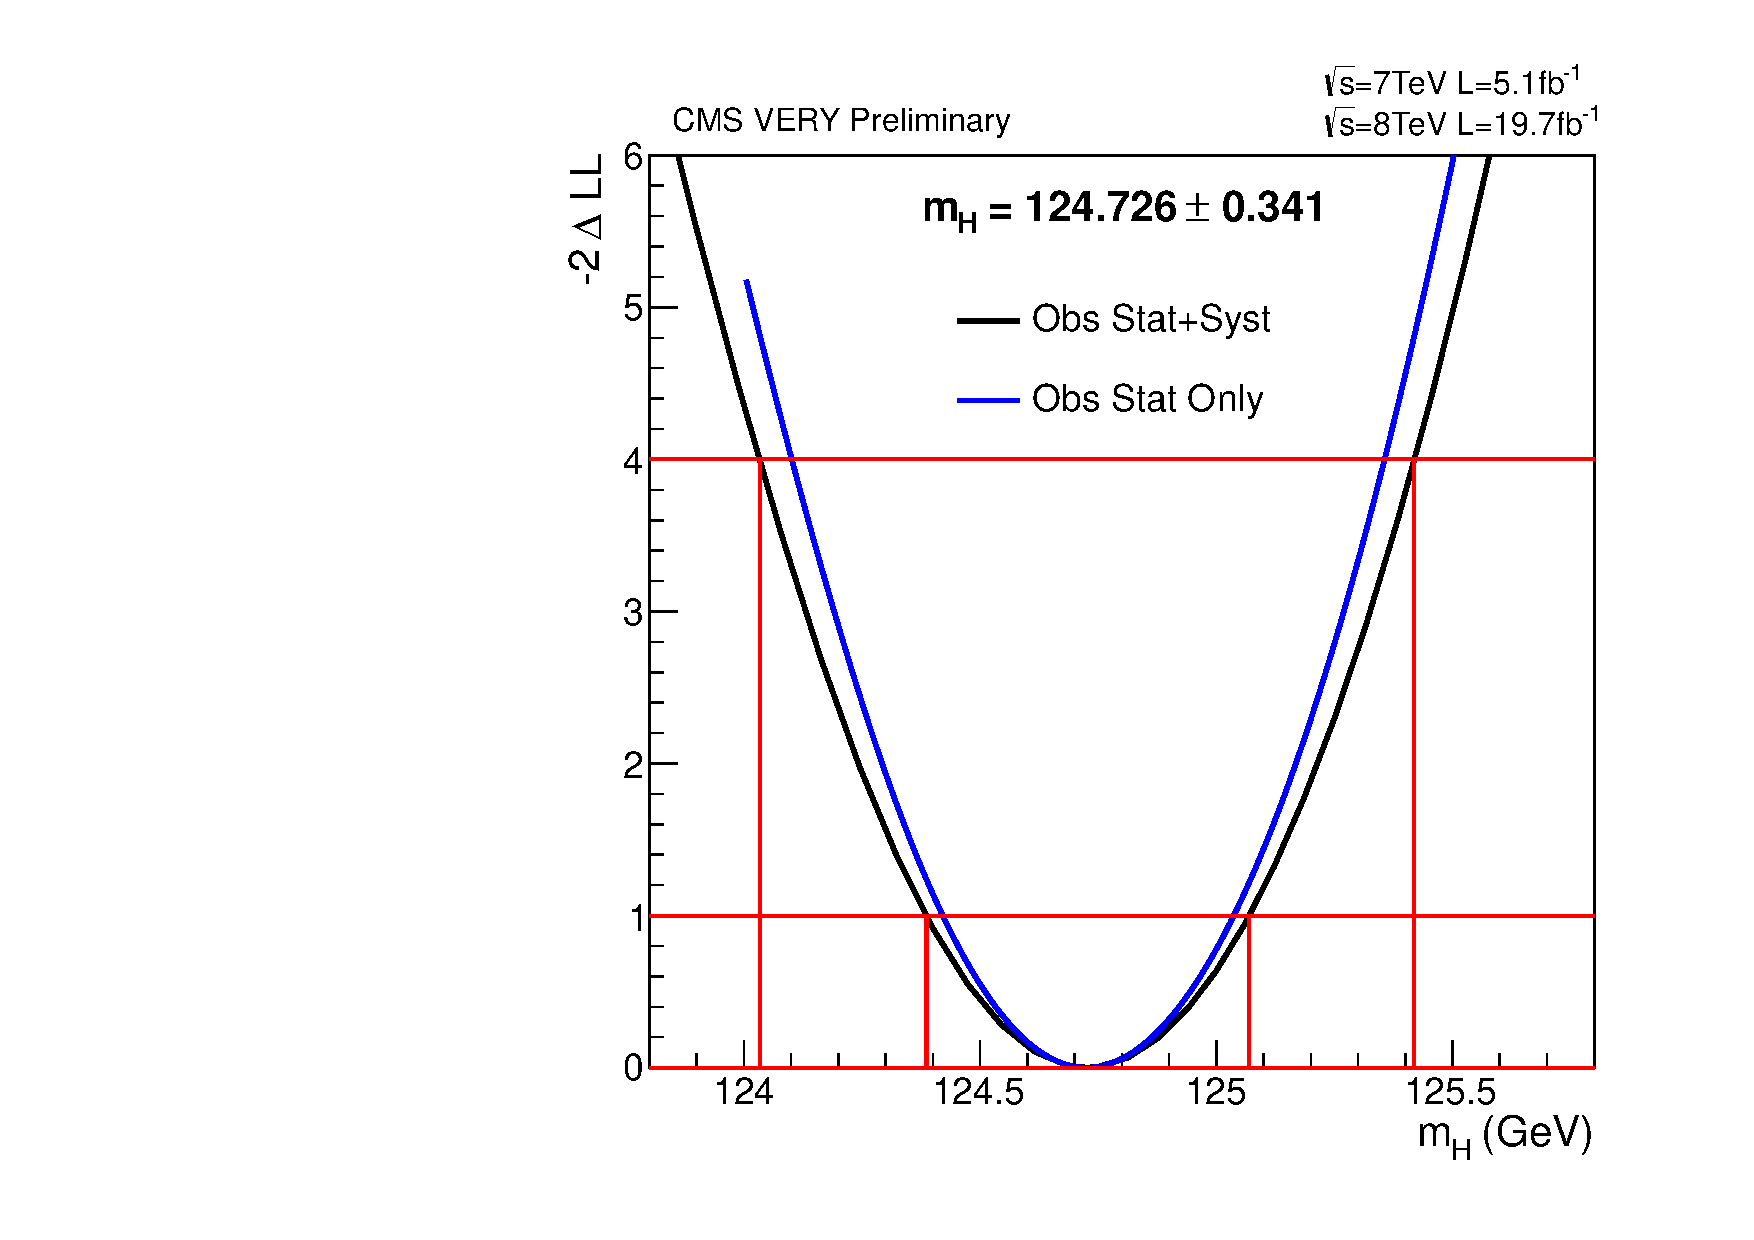
\includegraphics[width=0.49\textwidth]{analysis/plots/results/obsmh.pdf}
  \caption[2D \NLL scans of $\mu$ and \mH]{The two dimensional \NLL scan of $\mu$ and \mH when fitting to the combined 7+8~\TeV dataset is shown on the left. The best fit value is shown by the black cross and the $1\sigma$ and $2\sigma$ error contours shown by the solid and dashed lines respectively. The one dimensional \NLL scan of the best fit mass \mH is shown on the right, when profiling over the relative signal production from fermionic and bosonic modes, \RF and \RV. The statistical only component is shown as the blue line and the statistical plus systematic as the black line.}
  \label{fig:res_mumh2}
\end{figure}

Aside from the mass and signal strength of the observed particle it is relevant to study its couplings and whether the relative fraction produced by the different production modes is also compatible with the \SM prediction. Figure~\ref{fig:res_rvrf} (bottom left) shows the 2D \NLL scan of the relative couplings to fermions ($x$-axis) and bosons ($y$-axis) and their 1D projections (top left and top right). The \SM expectation is at (1,1) and represented by the dimond on the figure. It can be seen that the observation of $\mu_{ggH+tth}=X\pm\sigma$, $\mu_{qqH+VH}=X\pm\sigma$ is very compatible with the \SM expectation. Furthermore the signal strength can be divided by production mode as shown on the bottom right of Fig.~\ref{fig:res_rvrf}. It can be seen that the signal strength for all four production mechanism is consistent with the \SM expectation at 1. The Higgs mass, \mH, is profiled in all of these scans but constrained to be the same across each production mode.

\begin{figure}
  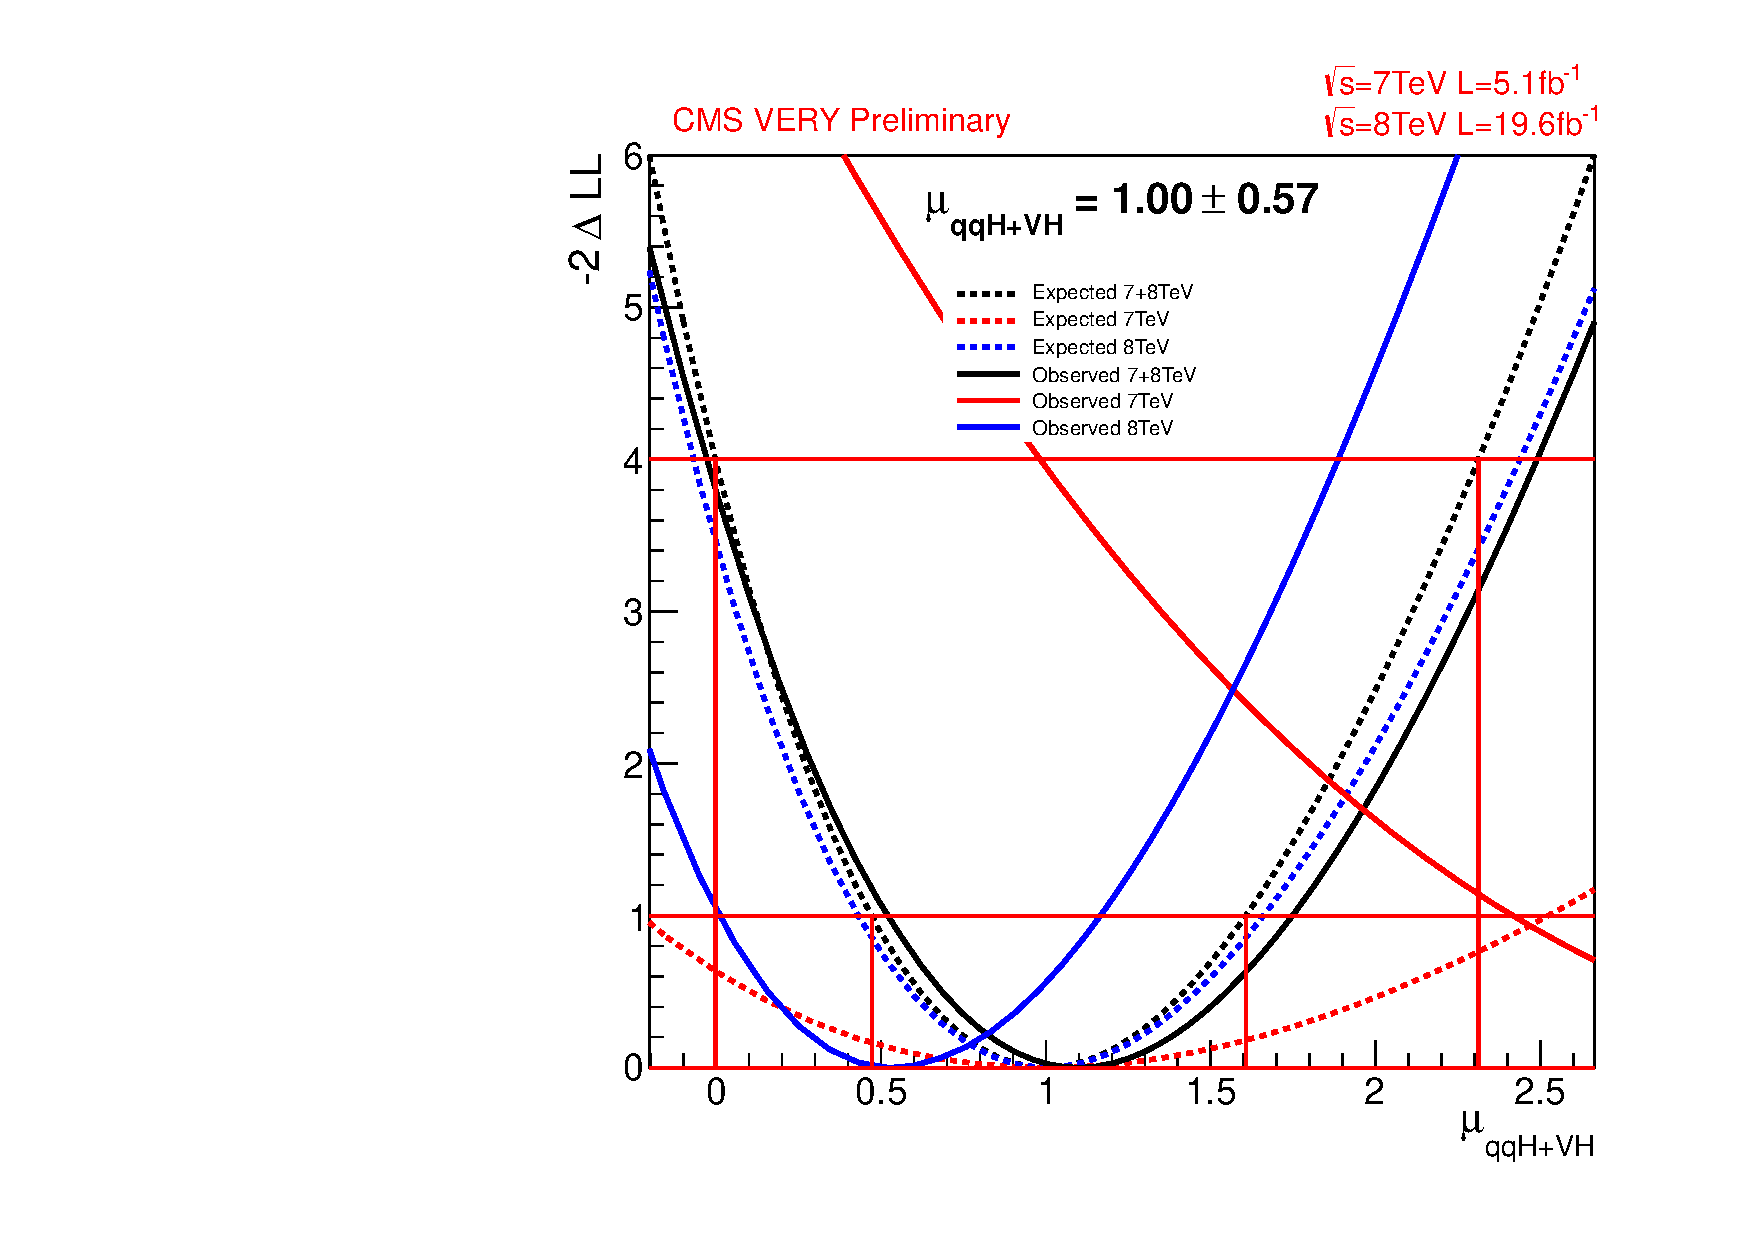
\includegraphics[width=0.49\textwidth]{analysis/plots/results/obsrv.pdf}
  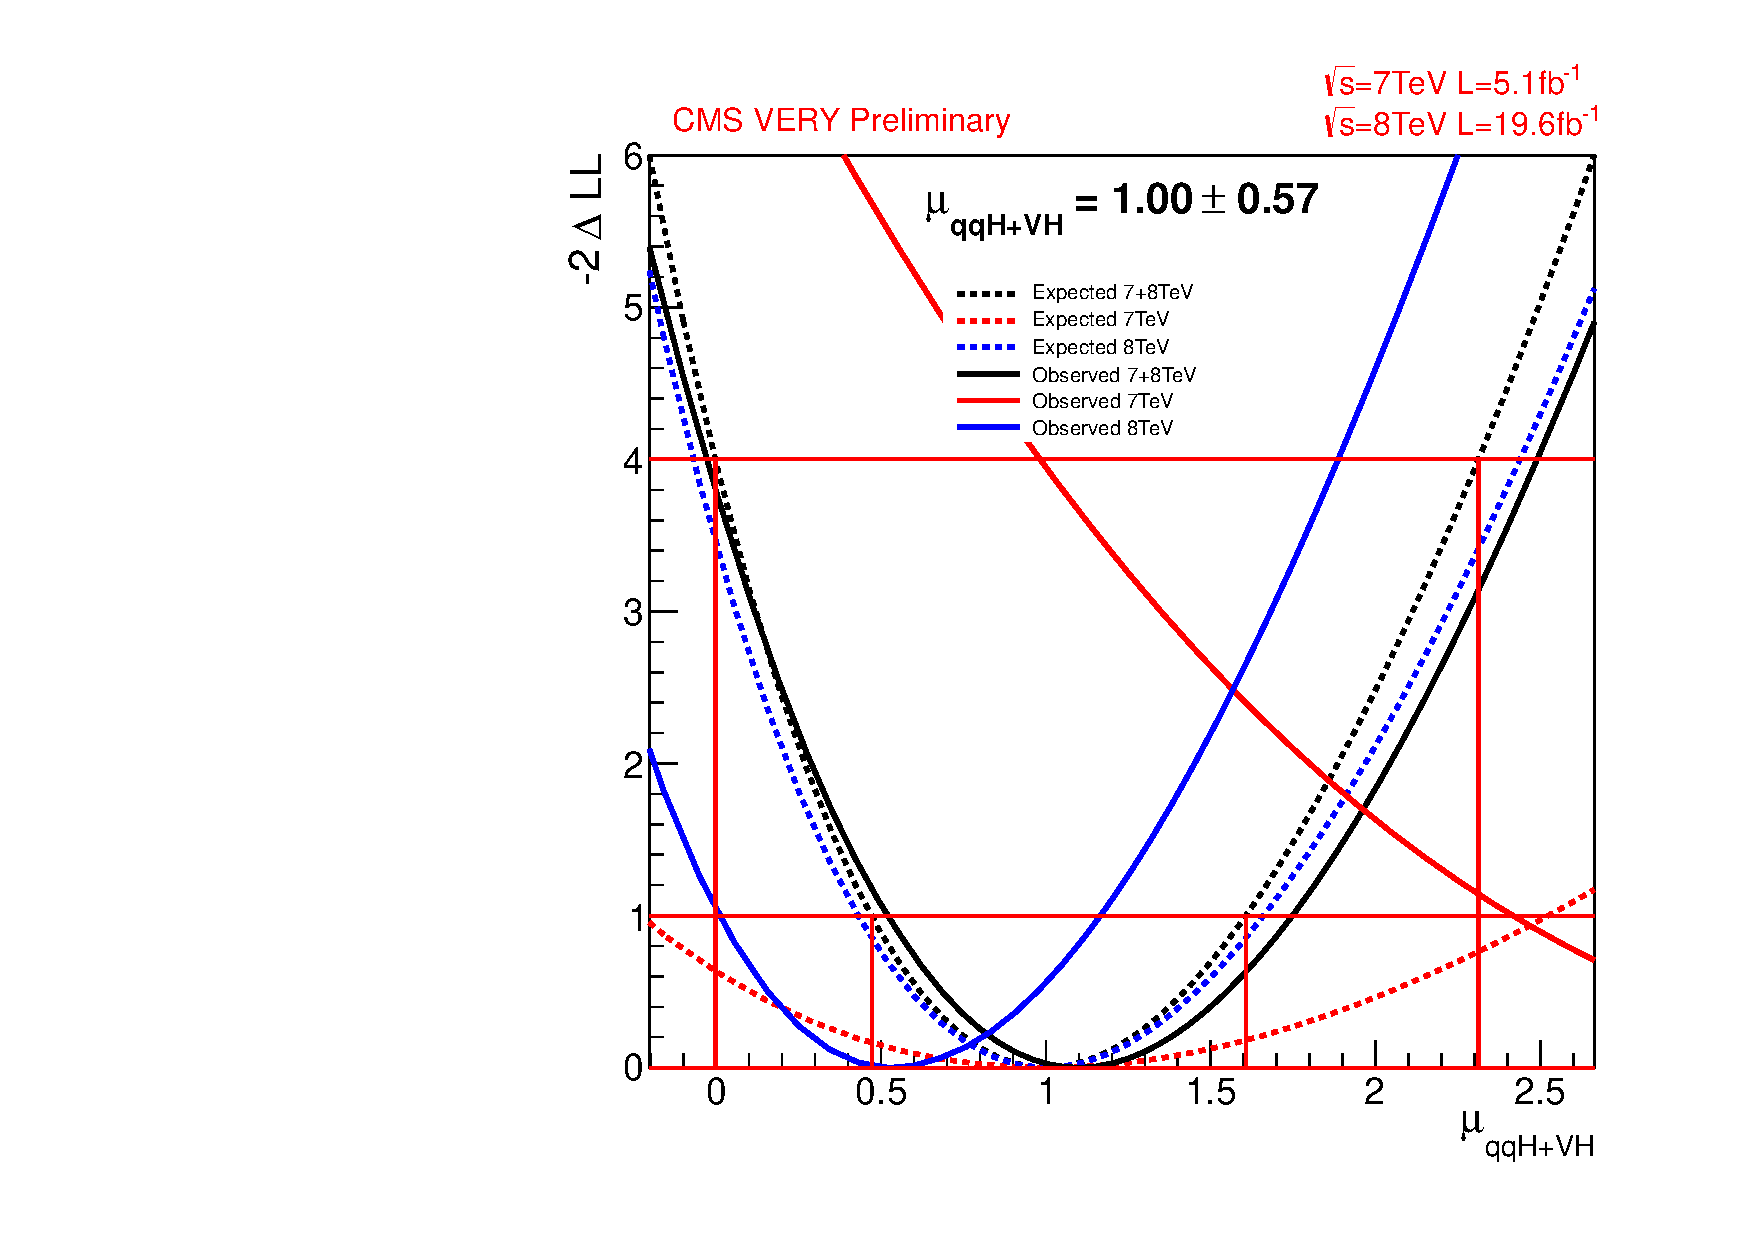
\includegraphics[width=0.49\textwidth]{analysis/plots/results/obsrf.pdf} \\
  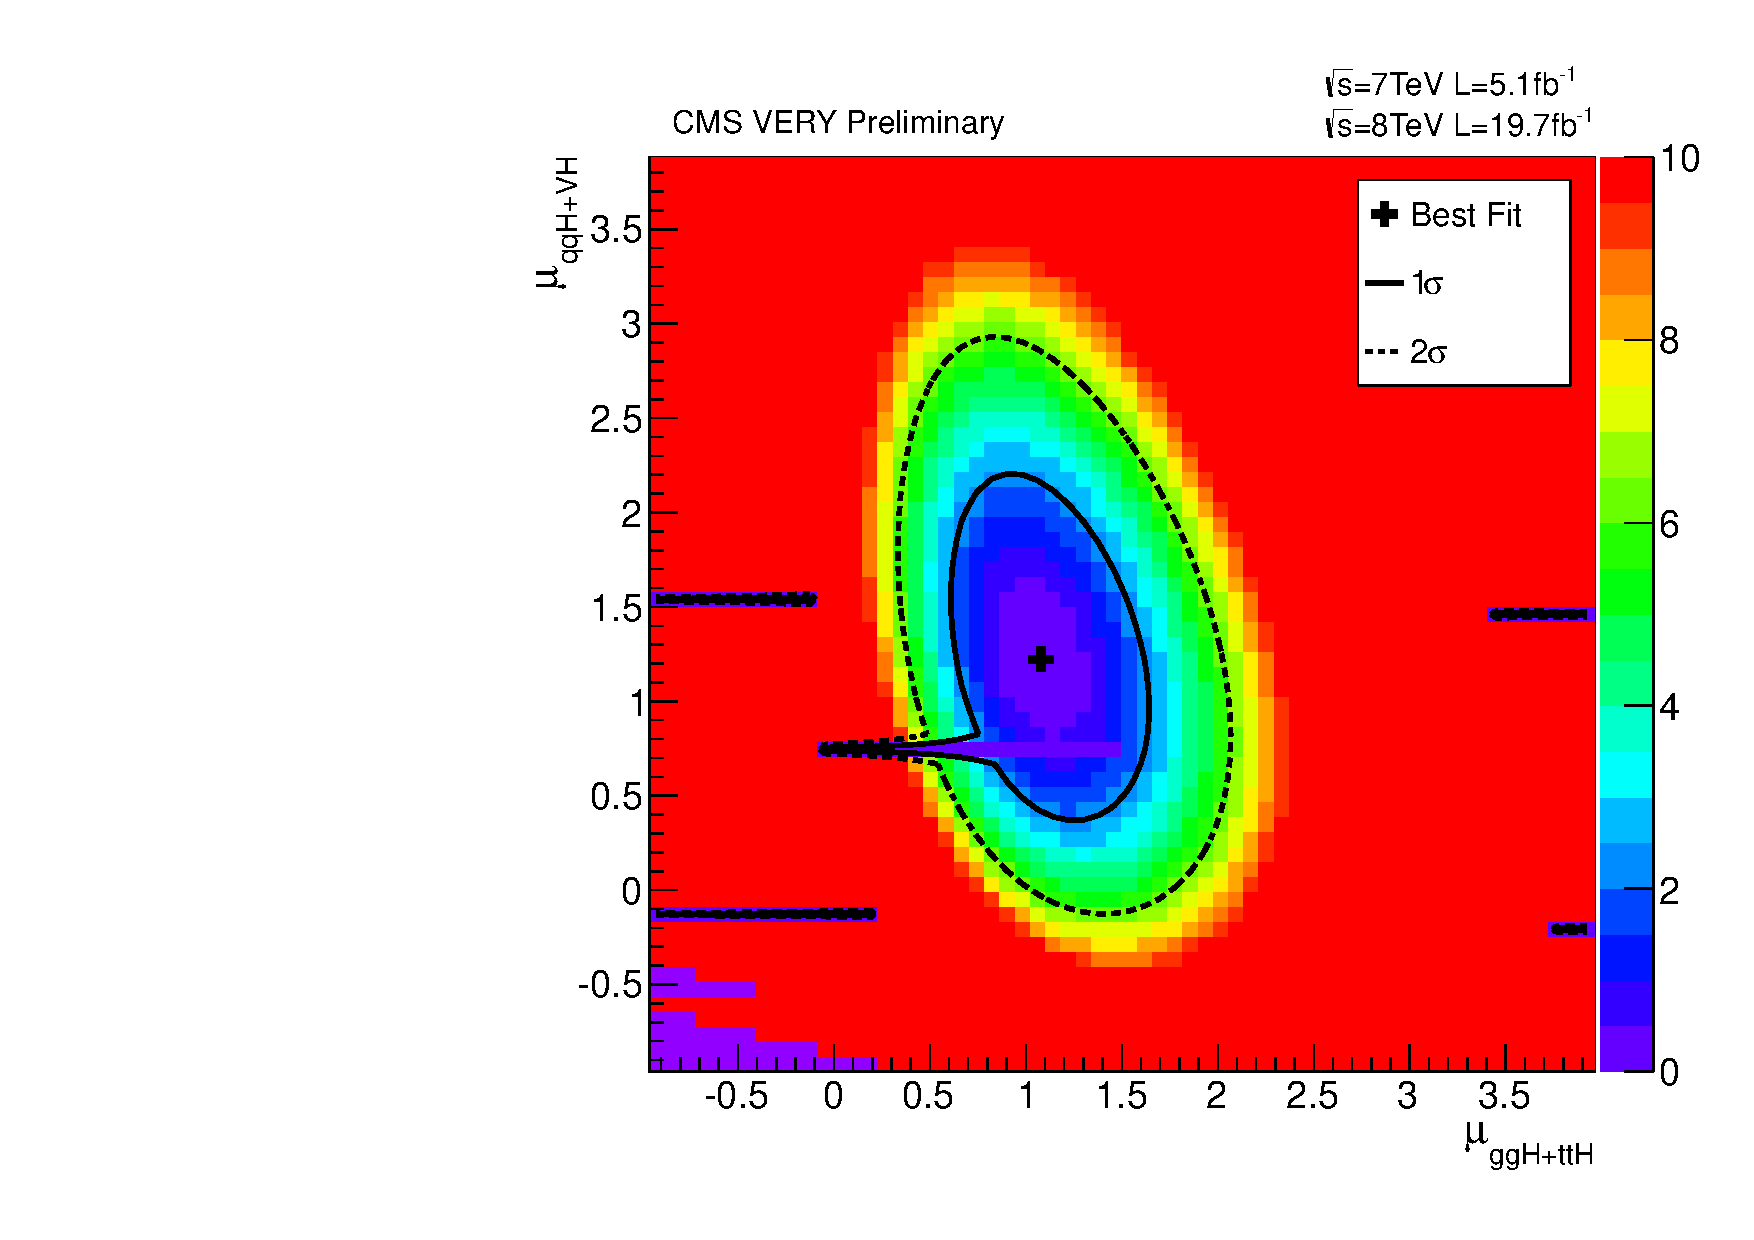
\includegraphics[width=0.49\textwidth]{analysis/plots/results/obsrvrf.pdf}
  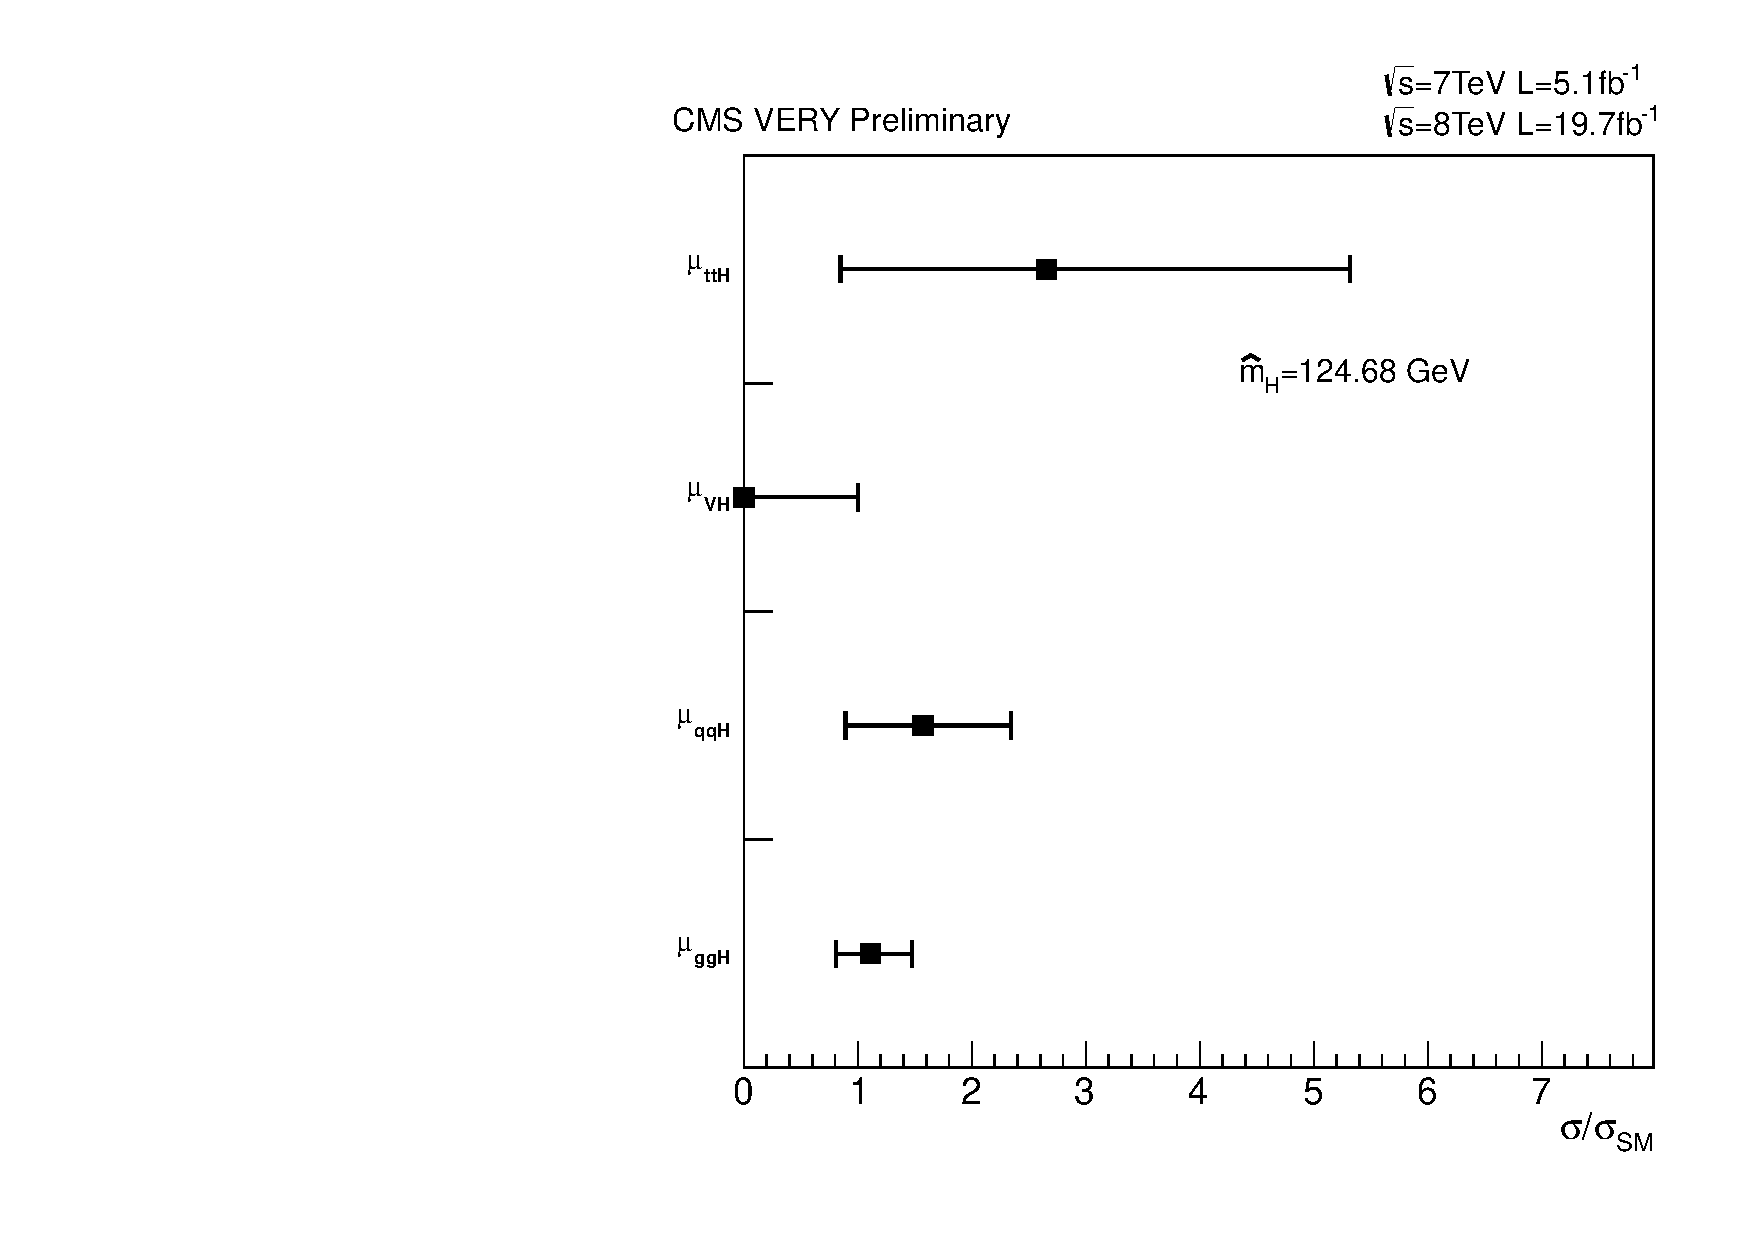
\includegraphics[width=0.49\textwidth]{analysis/plots/results/obsprocscan.pdf}
  \caption[Observed best fit values and \NLL scans of the observed bosons couplings to fermions and bosons respectively]{The top row shows the 1D \NLL scan as a function of the \SM relative coupling to bosons, $\mu_{qqH+VH}$ (top left), and to fermions, $\mu_{ggH+tth}$ (top right) for \SM expectation (dashed lines) and the observation in data (solid lines) for the 7~\TeV (red), 8~\TeV (blue) and combined (black) datasets. The bottom left plot is the 2D \NLL scan of $\mu_{qqH+VH}$ ($y$-axis) vs.~$\mu_{ggH+ttH}$ ($x$-axis) for the combined dataset observation. The best fit point is shown by the black cross whilst the $1\sigma$ and $2\sigma$ error intervals are shown by the solid and dashed lines respectively. The \SM expectation is the yellow diamond. It can be seen that the observation is very compatible with the \SM prediction.}
  \label{fig:res_rvrf}
\end{figure}

Figure ~\ref{fig:res_chcomp} shows the breakdown of the extracted signal strength when separately fitted for each of the analysis categories (left) and when grouping the categories by their topology (right) into those untagged, those which are dijet (or \VBF) tagged, \VH tagged or \ttH tagged. It is noticeable that the categories with the most sensitivty are the untagged categories especially the "Untagged 1" and "Untagged 2" at 8~\TeV, whilst the dijet categories also have considerable sensitivity given that the signal to background ratio is high. The \VH and \ttH tagged categories have the least sensitivty and whilst they do not contribute much to the error on the total signal yield they are important when measuring the couplings of the observed boson.

\begin{figure}
  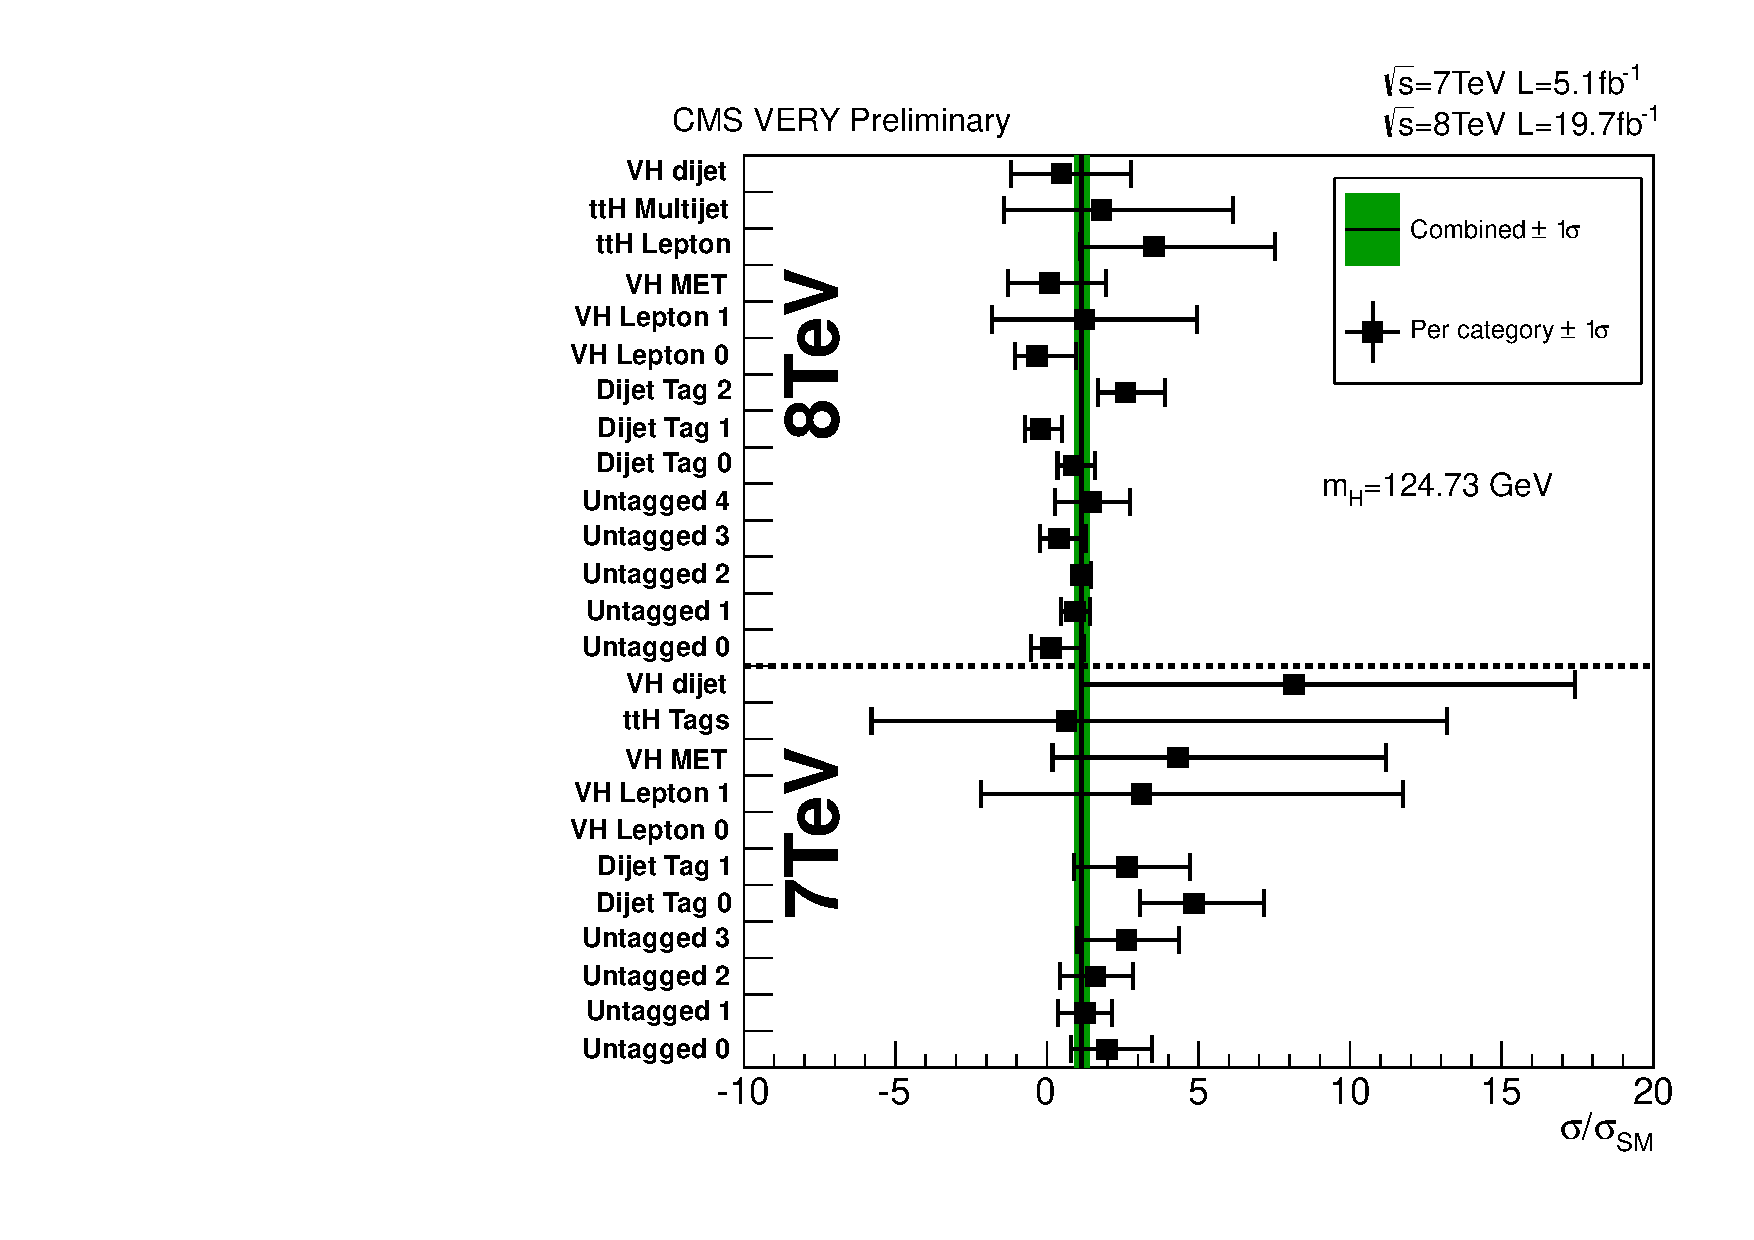
\includegraphics[width=0.49\textwidth]{analysis/plots/results/obschcomp.pdf}
  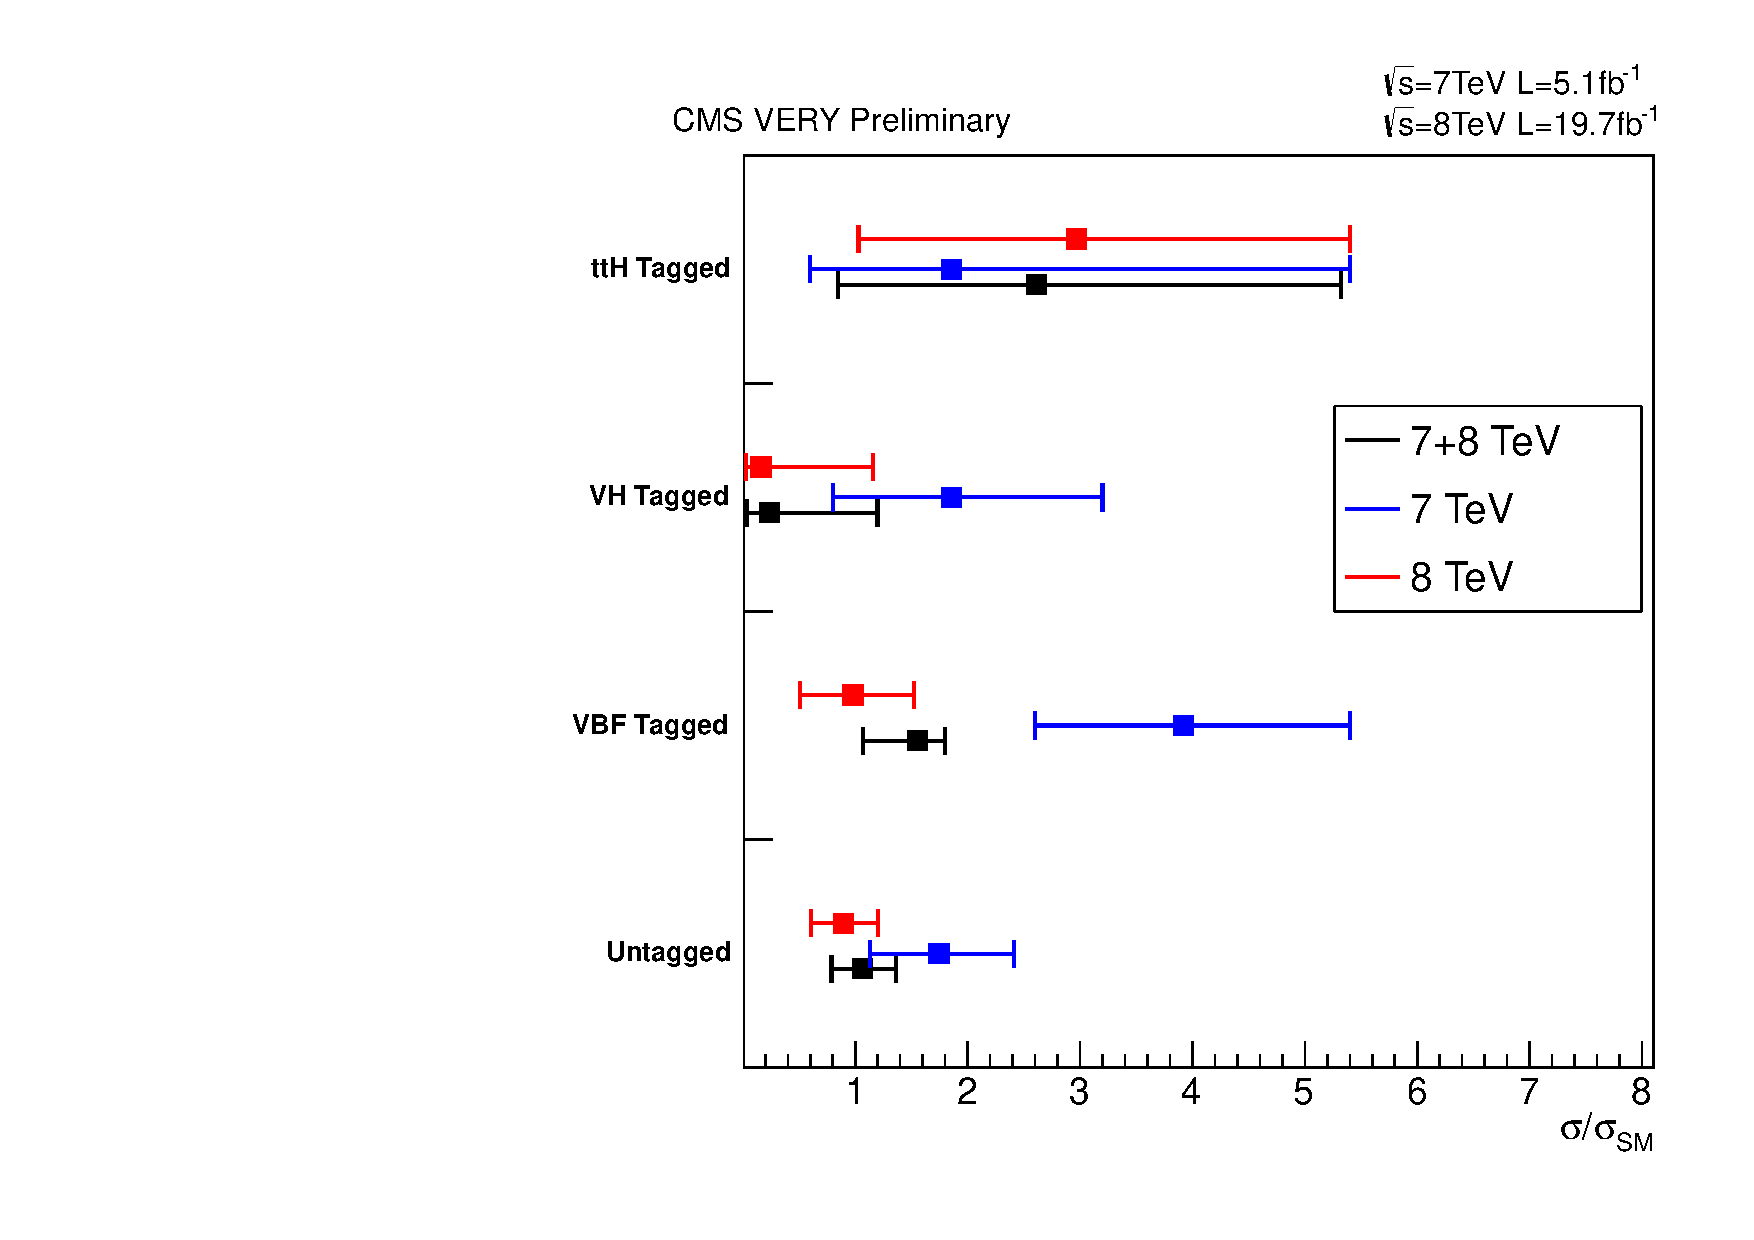
\includegraphics[width=0.49\textwidth]{analysis/plots/results/obstoposcan.pdf}
  \caption[The observed compatibility of the signal strength between channels]{The left plot shows the signal strength breakdown when fitting the signal strength, $\mu$, in each analysis category seperately. The right plot shows the signal strength breakdown when fitting categories split by their topology, the 7~\TeV dataset is shown in red, the 8~\TeV in blue and the combined dataset in black.}
  \label{fig:res_chcomp}
\end{figure}

These results show an independent discovery of the Higgs like state around 125~\GeV which was announced by the \CMS and ATLAS collaborations in 2012~\cite{CMSDiscovery,ATLASDiscovery}. Furthermore, measurements of the properties of the observed resonance in this decay channel indicate a particle very consistent with the \SM prediction.

\section{Spin}
\label{sec:spin_results}

The acceptance $\times$ efficiency of the two spin models in each category as well as the differential cross section as a function of \abscostheta, which depends only on the spin of the initial state, is obtained from the MC simulation. The only remaining assumption is on the total number of expected signal events for a given spin-parity state and production mode. This is well defined for the spin-0 SM case and is obtained from the $\sigma\times BR$ given by the LHC Higgs cross section working group in Ref.~\cite{LHCHiggsCrossSectionWorkingGroup3}. For the graviton-like \twomp this quantity is unknown. 
%Consequently, when generating pseduo-experiments for a particular model, the model is first fitted to the data to extract the relative shapes and normalisations of the signal and background. 
Consequently we scale the signal models for both spin hypotheses with a modifier, $\mu$, such that when $\mu=1$ and all \costhetastar information is ignored, the total number of expected signal events for the model in question is equivalent to the SM expectation. 
When generating pseduo-experiments for a particular model, the value of all the free parameters in the fit (including the signal nuisance parameters, the background shape parameters and the signal srength $\mu$) are set to their best fit values after fitting the model in question to the data.
In this way the expected separation is a fair representation of what we observe in data.

\subsection{SM compabibility check}
The signal yield, $\mu=\sigma/\sigma_{SM}$, is extracted independently in each of the \abscostheta bins, 
simultaneously fitting over the $\eta$ and \rnine bins such that the relative yields in each of the $\eta$ and \rnine 
bins is constrained to that predicted by the SM. The result is shown in Figure~\ref{fig:channelcomp} for the data (black points), the \zerop model expectation (red line), the \twomp model expectation using the $gg$ production mode only (blue line), the \twomp model expectation using the $q\bar{q}$ production mode only (green line) and the \twomp model expectation using a half-half mixture of $gg$ and $q\bar{q}$ production (magenta line), where for the expectations a single representative toy is used, obtained using asymptotic formulae from Ref.~\cite{asymptotic_form}, and the normalisation is extracted from a fit to data. The final point of the blue line can be understood
by referring back to Figure~\ref{fig:eff_acc}. The fact that the SM $ggH$ and $qqH$ production is of a similar strength at high values of \abscostheta causes the 
fitted strength (when fitting the \zerop model to the \twomp($gg$) expectation) to be smaller in the highest \abscostheta bin as compared to the second highest, contrary to what might be expected. 

\begin{figure}
  \begin{center}
    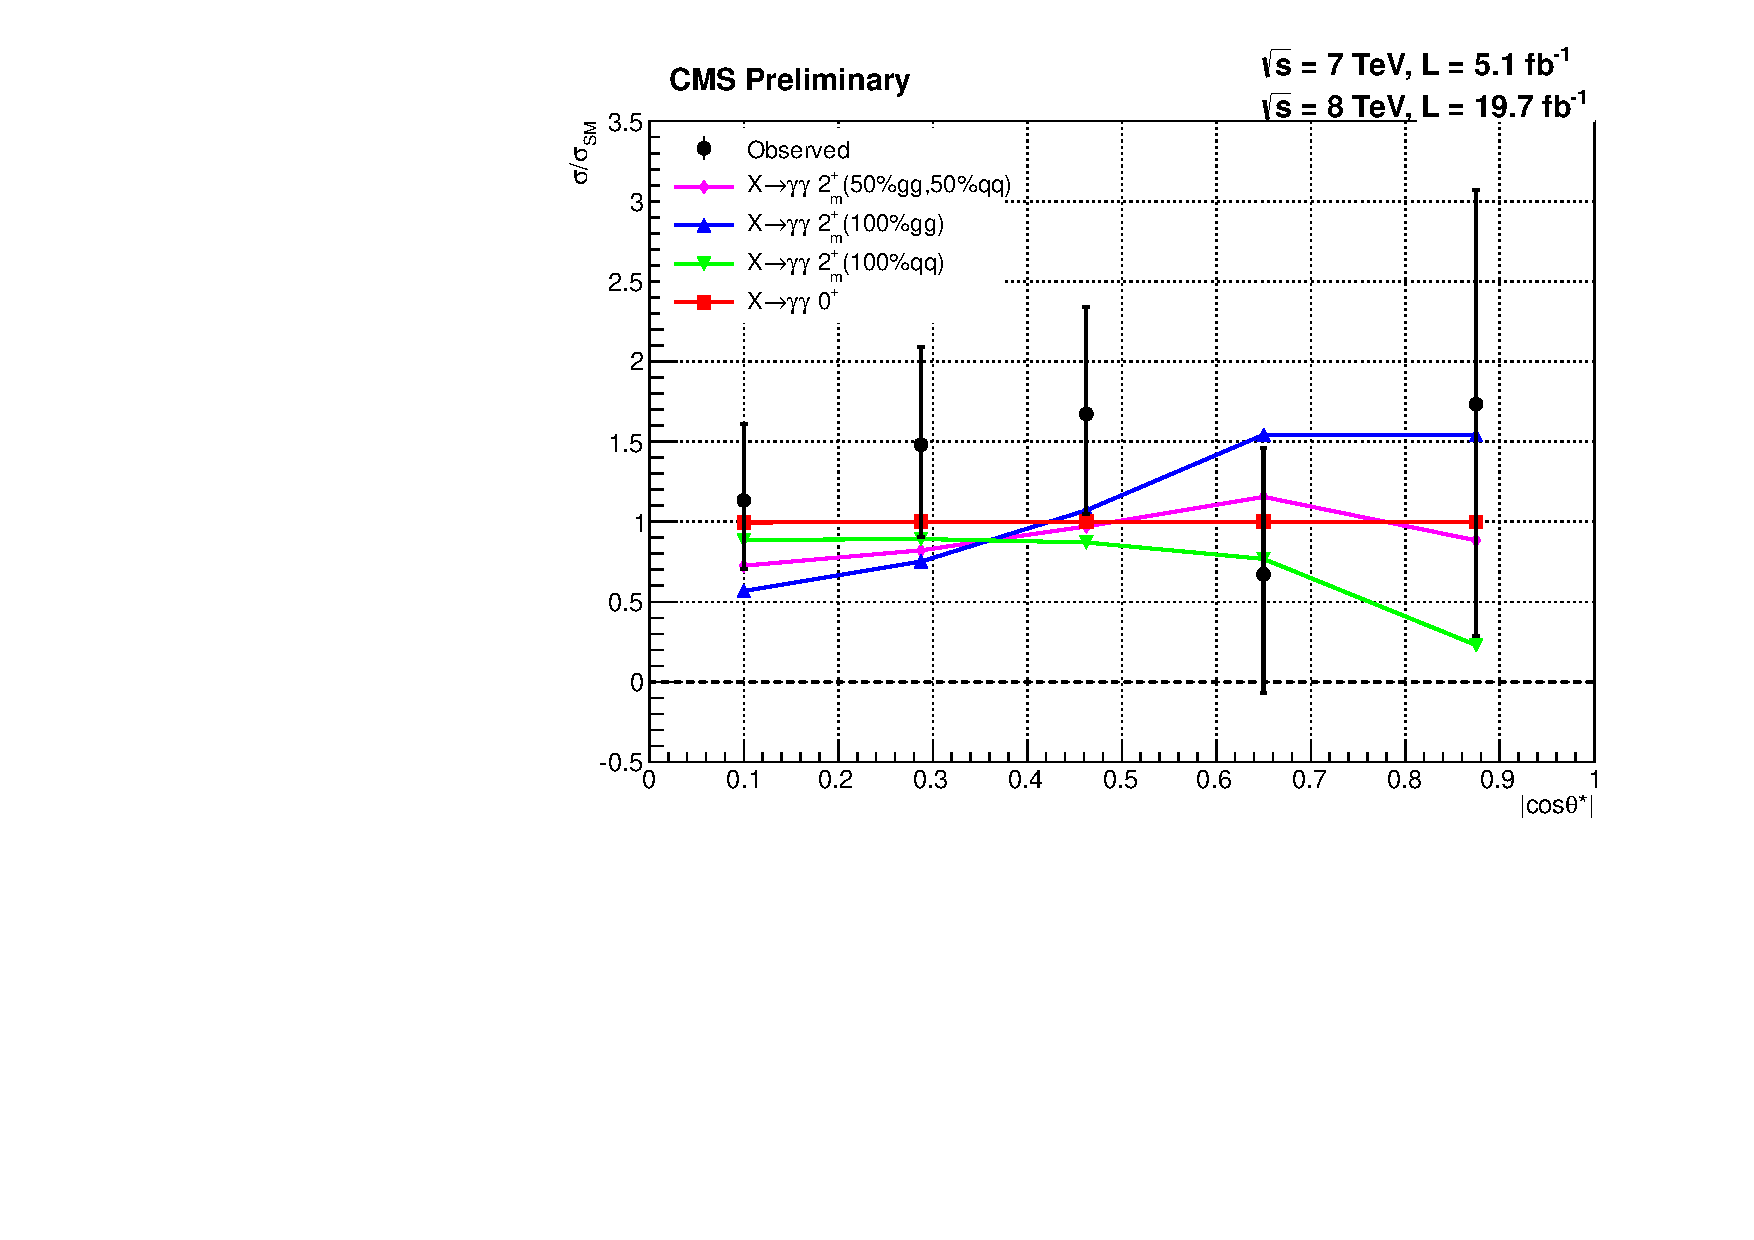
\includegraphics[width=0.8\linewidth]{spin/plots/ch_comp_multipdfcomb_unblind.pdf}
    \caption[The \SM signal strength extraction in bins of \abscostheta for the spin analyis]{The SM extracted signal yield as a function of \abscostheta for the \zerop expectation (red line), \twomp expectation with gluon-fusion production only (blue line), the \twomp expectation with quark-antiquark annihilation production only (green line), the \twomp expectation with half $gg$, half $q\bar{q}$ production (magenta line) and the observation (black points).}
    \label{fig:channelcomp}
  \end{center}
\end{figure}

\subsection{Hypothesis tests of the SM Higgs, \zerop, vs. graviton-like, \twomp}
\label{sec:spin_separation}

The separation between the two models and the data is extracted using the test statistic defined as twice the negative ratio 
of the likelihoods for the \zerop signal plus background hypothesis and the \twomp signal plus background hypothesis when 
performing a simultaneous fit of all twenty event classes together, $q=-2\,{\ln({\cal L}_{2^{+}_\mathrm{m} + \mathrm{bkg.}}/{\cal
L}_{0^+ + \mathrm{bkg.}})}$.

The distribution of this test statistic is shown in 
Fig.~\ref{fig:separation} for pseudoexperiments generated with an overall signal yield and signal position which is extracted from a fit to the data for
the \zerop hypothesis (orange) 
and the \twomp hypothesis (blue) for gluon-fusion production only (left) and quark-antiquark annihilation production only (right). The observed value is shown as the red arrow. The 1-$CL_{s}$ observed exclusion for a gluon-fusion only produced spin-2 boson is 93.7\% whilst for quark-antiquark produced boson is 85.0\%. 

\begin{figure}
  \begin{center}
    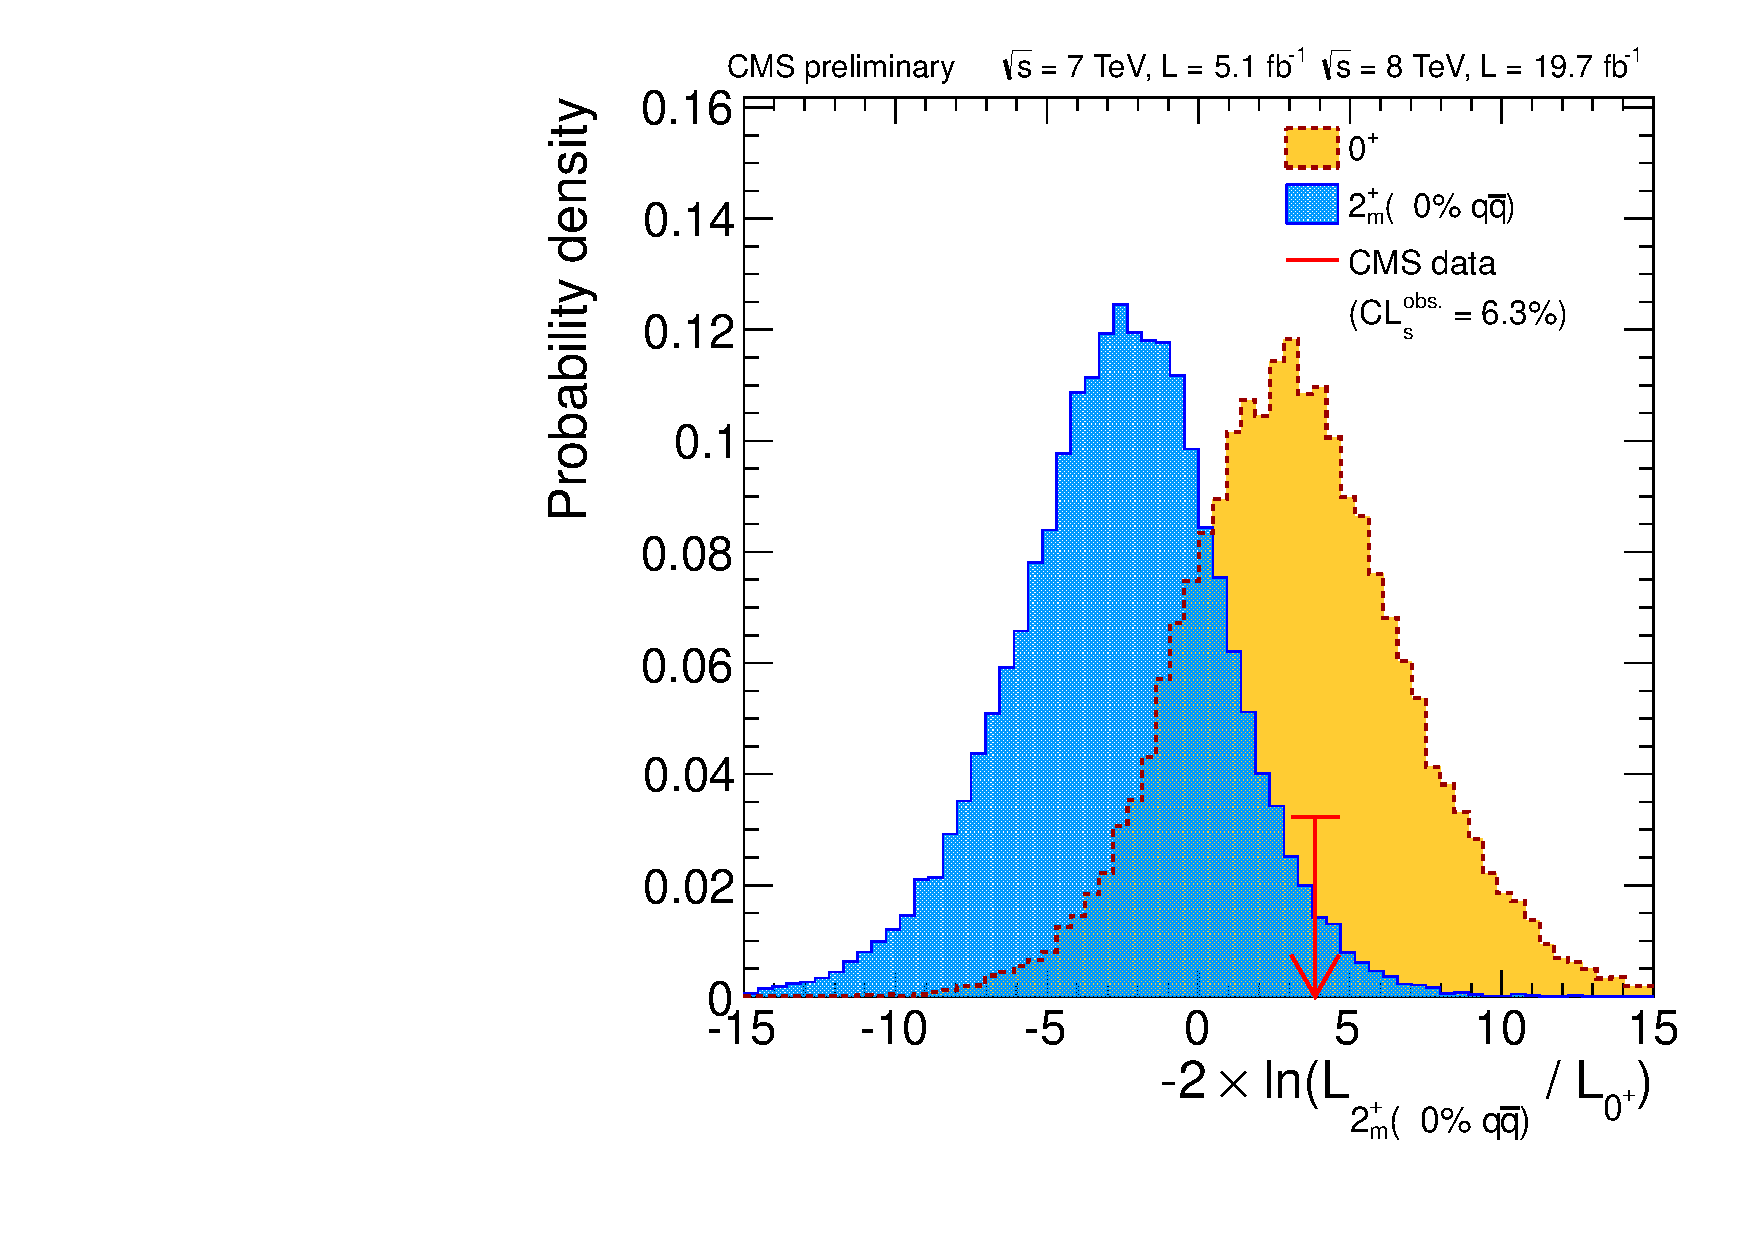
\includegraphics[width=0.49\linewidth]{{spin/plots/2pm0.00_unblind}.pdf}
    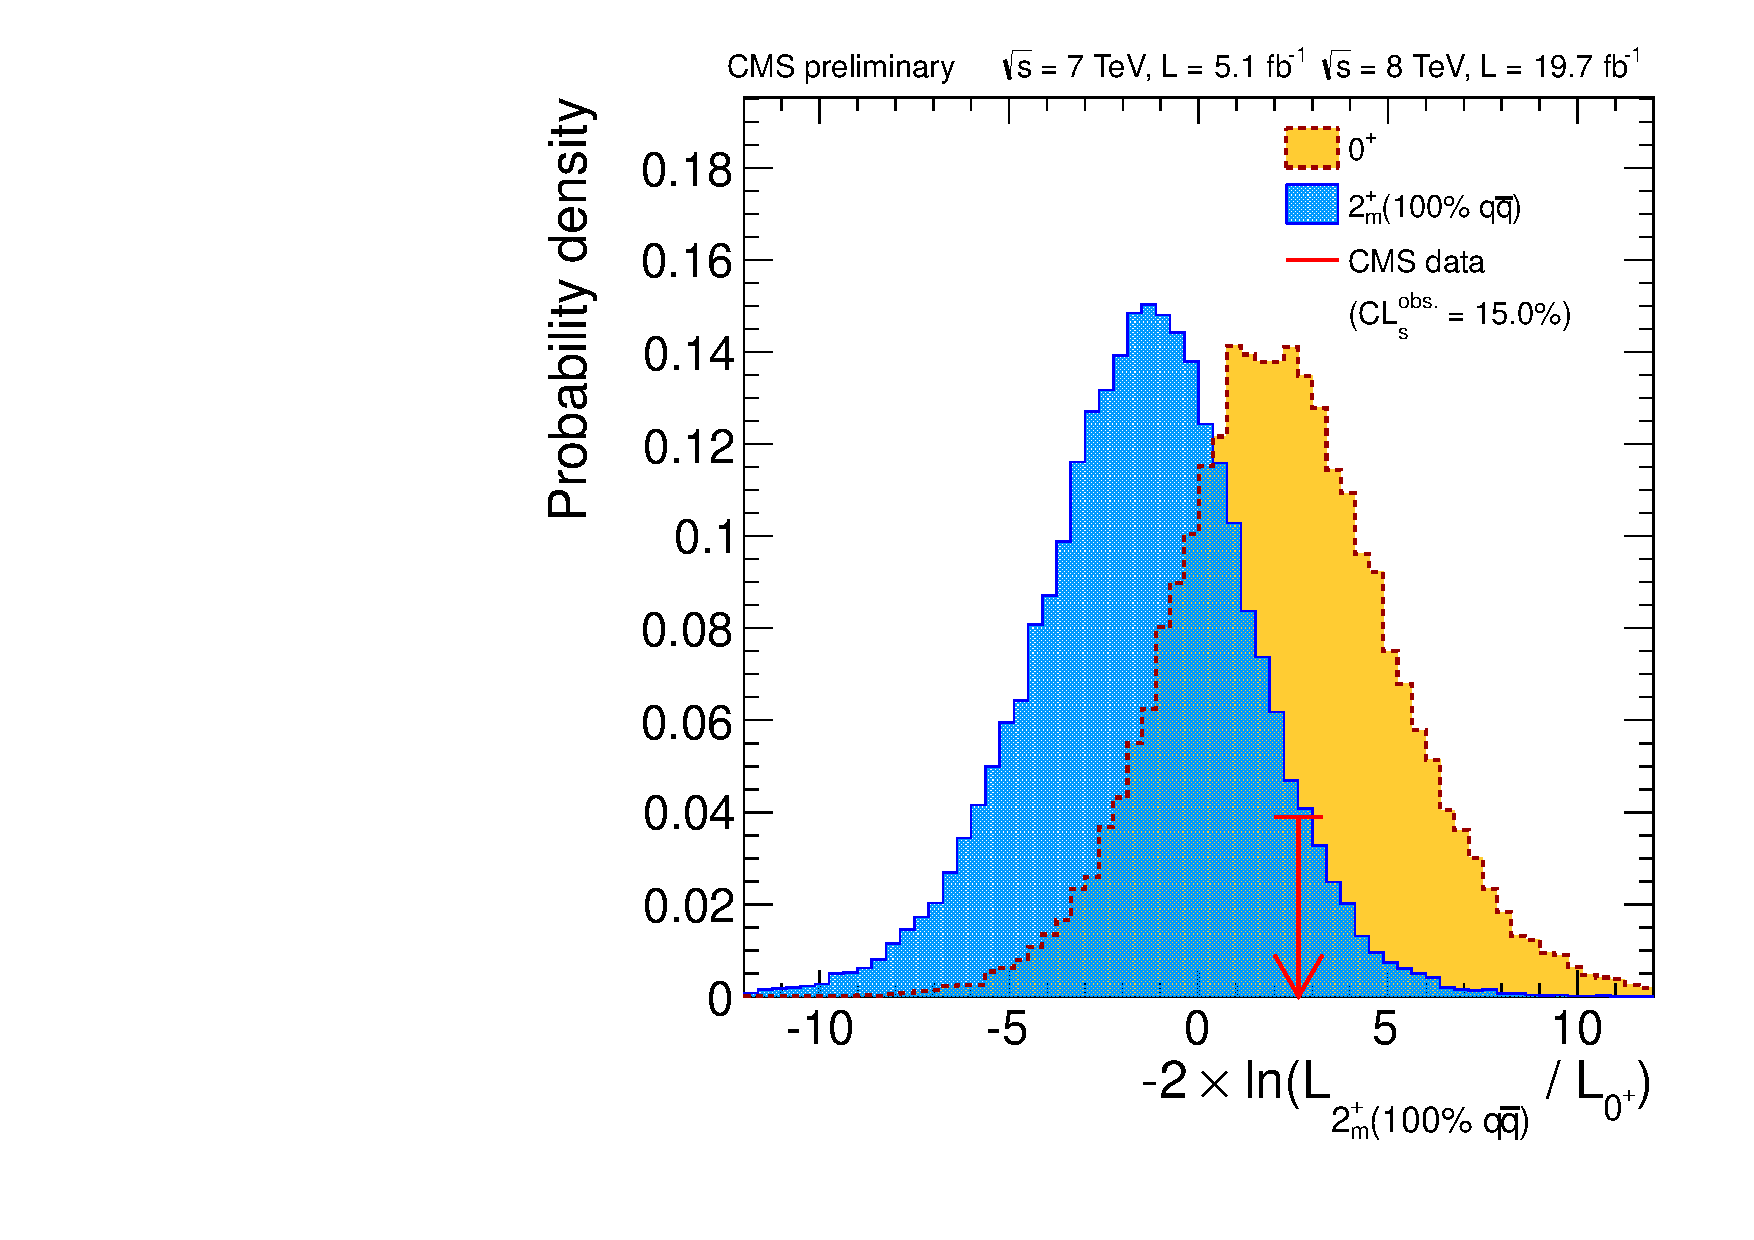
\includegraphics[width=0.49\linewidth]{{spin/plots/2pm1.00_unblind}.pdf}
    \caption[Distributions of the test statistic for different spin hypotheses compared to the \SM]{The distribution of the test statistic for pseudo experiments generated under the SM, \zerop, hypothesis (orange) and the \emph{graviton-like}, \twomp, hypothesis (blue) with gluon fusion produciton only (left) and quark-antiquark production only (right). The observed value in the data is shown as the red arrow.}
    \label{fig:separation}
  \end{center}
\end{figure}

The previous two tests are both performed assuming that the \twomp state is produced entirely by either gluon-fusion or quark-antiquark annihilation. A further three points, with mixtures of $gg$ and $q\bar{q}$ spin-2 production, have been tested such that the overall yield of the \twomp signal is fixed to the best fit value of the model in question to data and the fraction of \qqbar production is increased by a factor, \fqqbar. Figure~\ref{fig:qqbar} shows the distribution of the test statistic as a function of the fraction of \twomp production from $q\bar{q}$ annihilation. Figure~\ref{fig:separation} is, in effect, a projection of Fig.~\ref{fig:qqbar} at the points \fqqbar=0\% and \fqqbar=100\%. It can be seen that the data is very much in line with the \SM expectation. Whilst \textit{a prior} it may look as though the data points in Fig.~\ref{fig:qqbar} lie to close to the \SM mean (red line) all of these points are highly correlated. If the data look flat in \abscostheta then they will look flat for all values of \fqqbar. In this sense the green and yellow bands in Fig.~\ref{fig:qqbar} can be misleading.

\begin{figure}
  \begin{center}
    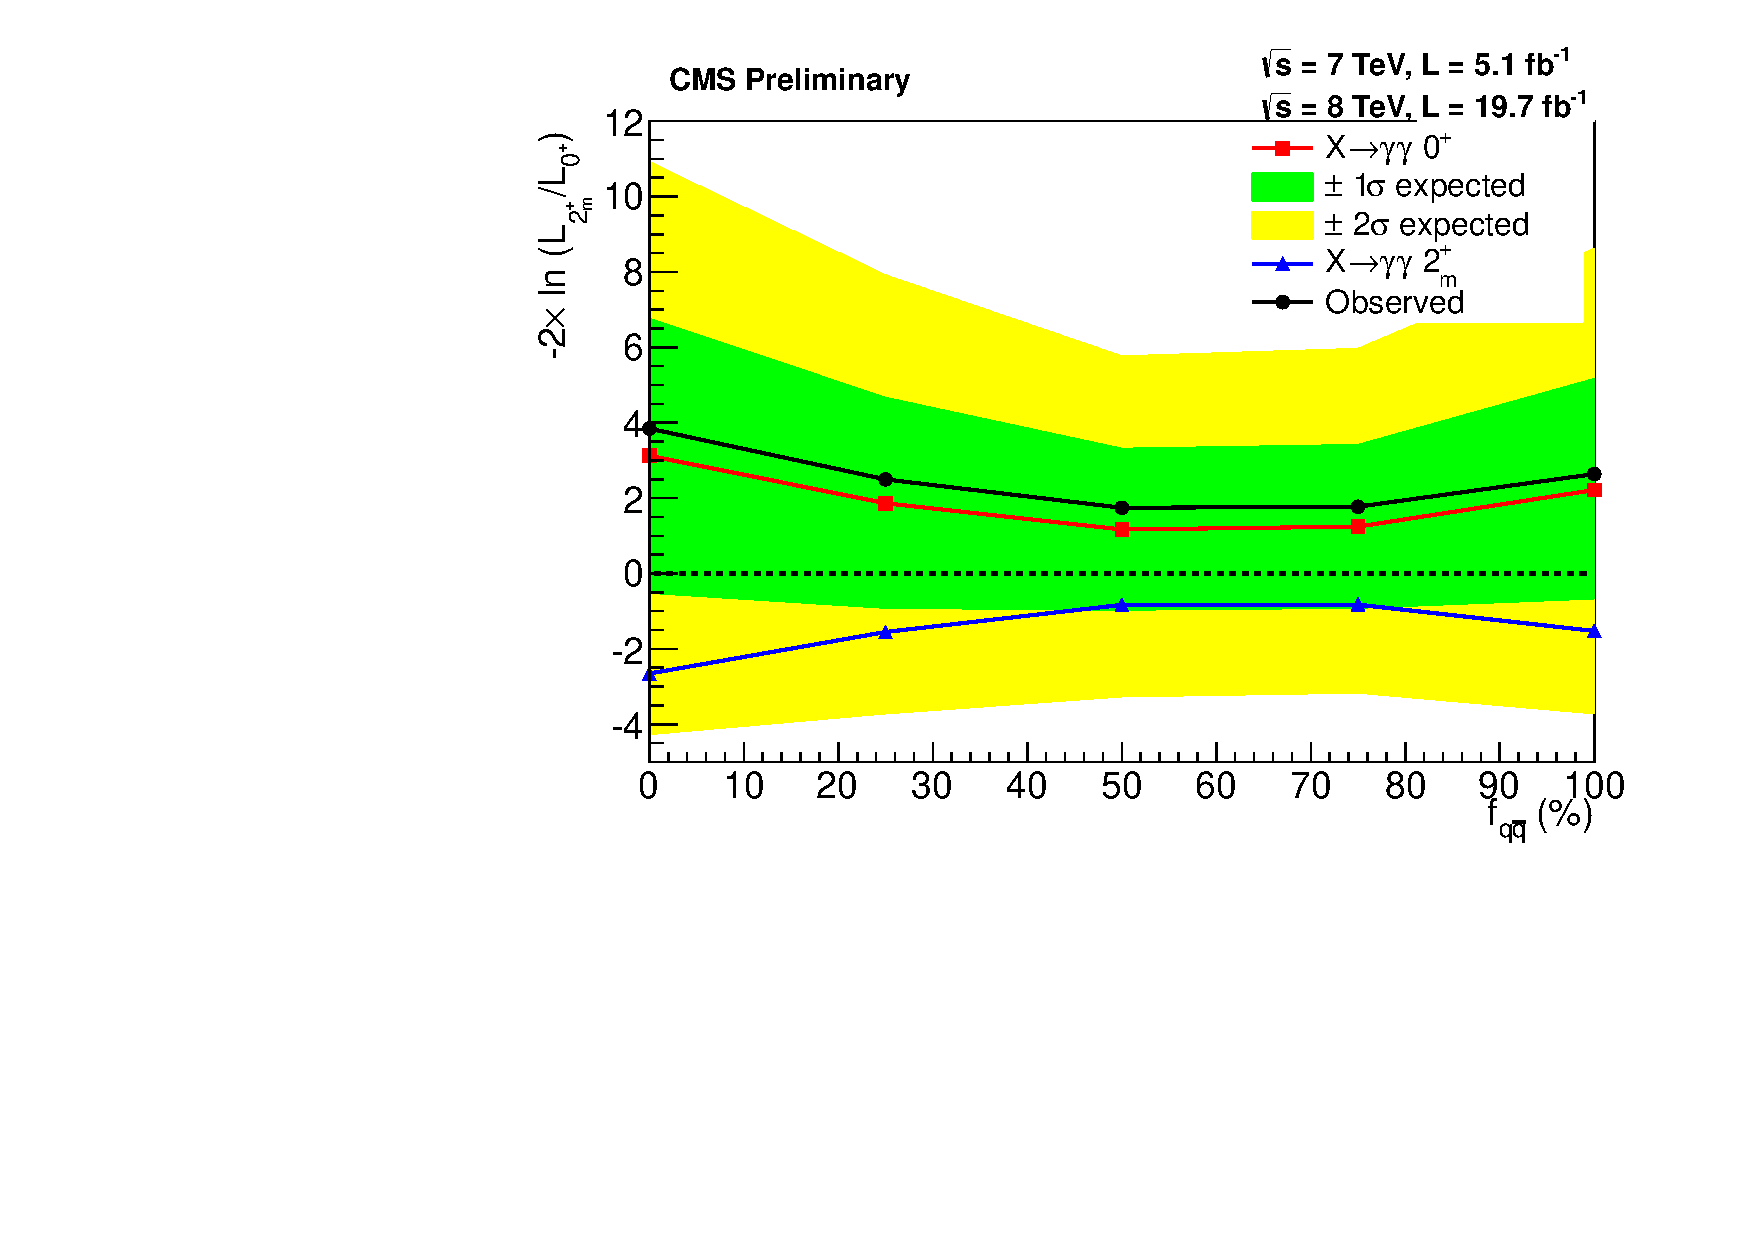
\includegraphics[width=0.8\linewidth]{spin/plots/fqqbar_unblind.pdf}
    \caption[Distribution of the test statistic as a function of \fqqbar for the spin analysis]{The distribution of the test statistic for pseudo experiments thrown under the SM, \zerop, hypothesis (red) and the \emph{graviton-like}, \twomp, hypothesis (blue) as a function of the fraction of \qqbar production relative to $gg$ production. The observed distribution in the data is shown by the black points.}
    \label{fig:qqbar}
  \end{center}
\end{figure}



